% MIT License
% 
% gitnote.tex
% 
% Copyright (c) 2020 冬ノ夜空
% 

\documentclass[10pt,a4j,openany,dvipdfmx]{jsarticle}
\usepackage{docmute} %for "input" command

  % -- page layput
  \usepackage[top=3cm, bottom=3cm, left=3.5cm, right=2cm, includefoot]{geometry}

  % -- page configuration
  \renewcommand{\baselinestretch}{0.95} %行送りの倍率
  \renewcommand{\figurename}{Fig. }
  \renewcommand{\tablename}{Table. }

  % \renewcommand{\prepartname}{\Huge{Part\,}}
  % \renewcommand{\postpartname}{}
  % \renewcommand{\prechaptername}{Chapter\,}
  % \renewcommand{\postchaptername}{}

  %% \setlength{\hoffset}{4.6mm}
  %% \setlength{\marginparwidth}{0mm}

  % -- HyperLink
  \usepackage{url}
  \usepackage[dvipdfmx,bookmarks=true,bookmarksnumbered=true,colorlinks=true,linkcolor=MidnightBlue,urlcolor=MidnightBlue]{hyperref}
%  \usepackage[dvipdfmx,bookmarks=true,bookmarksnumbered=true,colorlinks=true,linkcolor=MidnightBlue,citecolor=MidnightBlue,urlcolor=MidnightBlue]{hyperref}

  % -- font
  \usepackage{bm}       %Italicな太字にする
  \usepackage{ulem}     % underlining for emphasis
  \usepackage{ascmac}   % "itembox" environment etc.

  \usepackage[T1]{fontenc}
  \usepackage{lmodern}   % Latin Modern フォントを使う
  \usepackage{courier}   % Courier typewriter フォント

  \usepackage{pxjahyper} %しおり・タイトル等の日本語の文字化け防止
  \usepackage{natbib}    %citeの強化版
  \bibliographystyle{ametsoc2014}

  % -- graphics / color
  \usepackage{graphicx}
  \usepackage{color}
  \usepackage{multicol}
  \usepackage[dvipdfmx,svgnames]{xcolor} %色の指定のためのパッケージ
  % \usepackage[dvipdfmx,dvipsnames]{xcolor} %色の指定のためのパッケージ

  % -- figure
  \usepackage{here}

  \usepackage{lscape}    % 図や表の回転
  \usepackage{pdflscape} % 自動的にLandscapeのページのみ回転してくれる

  \usepackage{enumitem}  % item環境のconfig.
    \setlist[description]{parsep=0mm,topsep=1mm,leftmargin=5mm}
    \setlist[itemize]{parsep=0mm,topsep=1mm,leftmargin=5mm}

  %background-image(all pages => \***; specific page => \This***)
  \usepackage{wallpaper}

  % -- symbol
  \usepackage{textcomp} % 様々なシンボル(特殊文字)を利用
                        % °は \degree、℃は \celsius を使う

  % 丸数字
  \newcommand{\maru}[1]{\lower0.5ex\hbox{{\Large \textcircled{\scriptsize{\raise0.5ex\hbox{\normalsize #1}}}}}}



%=========================================
% \usepackage{tocbibind}
% This option loads package tocbibind if not already done and so list of figures and list of tables are also added in the toc
% \usepackage{dotocloa} % Add algrism list into toc

\usepackage{tikz}
\usepackage{pxpgfmark}
  \usetikzlibrary{fit,calc}

  \usetikzlibrary{shadings} %for shading frame

%define a marking command
\newcommand*{\tikzmk}[1]{
\tikz[remember picture,overlay,] \node (#1) {};\ignorespaces
}

%define a boxing command, argument = colour of box
\newcommand{\boxit}[1]{
\tikz[remember picture,overlay]{\node[yshift=3pt,fill=#1,opacity=.25,fit={(A)( $(B)+(.95\linewidth,.8\baselineskip)$ )}] {};}\ignorespaces
}

%=========================================
% tcolorbox

\usepackage{tcolorbox}
  \tcbset{boxrule=0.3mm,left=1mm,right=1mm,top=1mm,bottom=1mm,boxsep=1.5mm}
  \newcommand{\defaultset}{\tcbset{colframe=Black!70!White,colback=White}}\defaultset

% newcommnd operation for tcolorbox
\newtcolorbox{forsomeone}[1]{fonttitle=\sffamily,title=#1}
\newtcbox{term}{colback=Red!10,left=1mm,right=1mm,top=1mm,bottom=1mm,before skip=2mm, after skip=2mm}\newcommand{\terminal}[1]{\texttt{\term{#1}}} %別行のターミナルコマンド
\newtcbox{inlineterm}{on line, colframe=Red!50!White, colback=Red!10,left=0.5mm,right=0.5mm,top=0.5mm,bottom=0.5mm,left skip=0.5zw, right skip=0.5zw,boxrule=0.2mm}\newcommand{\ilterm}[1]{\texttt{\inlineterm{#1}}} %行内のターミナルコマンド

\tcbuselibrary{listings}
% \newtcblisting{myverbatim}{listing only,colback=Black!5,before skip=2mm, after skip=2mm}
% \newtcblisting{multiterm}{listing only,colback=Red!10,before skip=2mm, after skip=2mm}

%\tcbuselibrary{skins}
\tcbuselibrary{many}

\newenvironment{blueitemize}{\begin{itemize}}{\end{itemize}}
\tcolorboxenvironment{blueitemize}{blanker,
left skip=10pt,left=10mm,
before skip=6pt,after skip=6pt,
borderline west={3mm}{0pt}{DeepSkyBlue}}


% \tcbset{skin=enhanced,fonttitle=\bfseries,
% frame style={upper left=Blue,upper right=Red,lower left=Yellow,lower right=Green},
% interior style={white,opacity=0.5},
% segmentation style={black,solid,opacity=0.2,line width=1pt}}

% \begin{tcolorbox}[title=Nice box in rainbow colors]
% With the 'enhanced' skin, it is quite easy to produce fancy looking effects.
% \tcblower
% Note that this is still a \texttt{tcolorbox}.
% \end{tcolorbox}

\makeatletter
  \newtcolorbox{picturebox}[2][]{%
  skin=enhanced, boxrule=1.0mm, fonttitle=\bfseries, 
  frame hidden, interior hidden, 
  overlay={\begin{tcbclipframe}\node at (frame)
  {\includegraphics[width=\tcb@width,height=\tcb@height]{#2}};\end{tcbclipframe}
  \begin{tcbclipinterior}\fill[white,opacity=0.75]
  (frame.south west) rectangle (frame.north east);\end{tcbclipinterior}},#1}
\makeatother


\newenvironment{oceanbox}[1]{\tcolorbox[savedelimiter=oceanbox,
skin=enhanced,boxrule=1.0mm,fonttitle=\bfseries,
frame style={upper left=Black,upper right=White,lower left=DeepSkyBlue,lower right=MidnightBlue},
interior style={white,opacity=0.5},
segmentation style={black,solid,opacity=0.2,line width=1pt},
title=#1]
} {\endtcolorbox}

\newenvironment{skybox}[1]{\tcolorbox[savedelimiter=skybox,
skin=enhanced,boxrule=1.0mm,fonttitle=\bfseries,
frame style={upper left=Black,upper right=White,lower left=Cyan,lower right=DodgerBlue},
interior style={white,opacity=0.5},
segmentation style={black,solid,opacity=0.2,line width=1pt},
title=#1]
} {\endtcolorbox}

\newenvironment{redbox}[1]{\tcolorbox[savedelimiter=redbox,
skin=enhanced,boxrule=1.0mm,fonttitle=\bfseries,
frame style={upper left=DarkRed,upper right=White,lower left=Black!50!DarkRed,lower right=Maroon},
interior style={white,opacity=0.5},
segmentation style={black,solid,opacity=0.2,line width=1pt},
title=#1]
} {\endtcolorbox}

\newtcolorbox{ColorReferenceBox}[1]{textmarker/.style={%
skin=enhancedmiddle jigsaw,breakable,parbox=false,
boxrule=0mm,leftrule=3mm,rightrule=3mm,boxsep=0mm,arc=0mm,outer arc=0mm,
left=3mm,right=3mm,top=1mm,bottom=1mm,toptitle=1mm,bottomtitle=1mm},
textmarker,colback=#1!5!white,colframe=#1}

% listing with line number
\newtcblisting{numList}[1]{
colback=red!5!white,colframe=red!25,
left=6mm, listing only,
listing options={style=tcblatex,language=#1,numbers=left,numberstyle=\tiny\color{red!75!black}}}

%=========================================
% commandshell, commandbox

  % color definition
  \definecolor{gentooblack}{HTML}{333333}
  
  % root user shell
  % *** Caution: 日本語を扱うのが苦手のよう!!!***
  \newtcblisting{rootshell}{boxrule=0.1mm,
  colback=gentooblack,colupper=white,colframe=DeepSkyBlue!95!white,
  listing only,listing options={style=tcblatex,language=sh},
  every listing line={\textcolor{red}{\small\ttfamily\bfseries [root]\# }}}
  
  % normal user shell
  % *** Caution: 日本語を扱うのが苦手のよう!!!***
  \newtcblisting{commandshell}{boxrule=0.1mm,
  colback=gentooblack,colupper=white,colframe=DeepSkyBlue!95!white,
  listing only,listing options={style=tcblatex,language=sh,columns=fullflexible,keywordstyle=\color{cyan}},
  every listing line={\textcolor{red}{\small\ttfamily\bfseries [user]\$ }}}

  \newtcblisting{onecommandshell}{boxrule=0.1mm,
  colback=gentooblack,colupper=white,colframe=DeepSkyBlue!95!white,
  listing only,listing options={style=tcblatex,columns=fullflexible}}

  % \usepackage{listings} or \tcbuselibrary{listings}
  \DeclareTotalTCBox{\commandbox}{ s v }
  {verbatim,colupper=white,colback=black!75!white,colframe=black}
  {\IfBooleanTF{#1}{\textcolor{red}{\ttfamily\bfseries > }}{}%
  \lstinline[language=command.com,keywordstyle=\color{cyan!35!white}\bfseries]^#2^}

%=========================================

% for drawing the git flow diagram
\usepackage{filecontents} 
\newcommand\commit[2]{\node[commit] (#1) {}; \node[clabel] at (#1) {\texttt{#1}: #2};}
\newcommand\ghost[1]{\coordinate (#1);}
\newcommand\connect[2]{\path (#1) to[out=90,in=-90] (#2);}

%=========================================

\usepackage{listings}
\lstset{
  language = , %プログラム言語(複数の言語に対応,C,C++も可)(plain textの場合は言語設定を空にする!!!)
  %backgroundcolor={\color{White}},                   %背景色と透過度
  breaklines = true,                                 %枠外に行った時の自動改行
  breakindent = 10pt,                                %自動改行後のインデント量(デフォルトでは20[pt])
  basicstyle = \ttfamily\scriptsize,                 %標準の書体
  commentstyle = {\itshape \color[cmyk]{1,0.4,1,0}}, %コメントの書体
  classoffset = 0,                                   %関数名等の色の設定
  keywordstyle = {\bfseries \color[cmyk]{0,1,0,0}},  %キーワード(int, ifなど)の書体
  stringstyle = {\ttfamily \color[rgb]{0,0,1}},      %表示する文字の書体
  %frame = TBrl,       %枠 "t"は上に線を記載, "T"は上に二重線を記載 
                       %他オプション:leftline,topline,bottomline,lines,single,shadowbox
  framesep = 5pt,      %frameまでの間隔(行番号とプログラムの間)
  numbers = none,      %行番号の位置 (行番号無し:none; 左:left; 右:right)
  stepnumber = 1,      %行番号の間隔
  numberstyle = \tiny, %行番号の書体
  tabsize = 4,         %タブの大きさ
  captionpos = t       %キャプションの場所("tb"ならば上下両方に記載)
}
%% Color Numbers
%\lstset
%{
%    literate=%
%    {0}{{{\color{Orange}0}}}1
%    {1}{{{\color{Orange}1}}}1
%    {2}{{{\color{Orange}2}}}1
%    {3}{{{\color{Orange}3}}}1
%    {4}{{{\color{Orange}4}}}1
%    {5}{{{\color{Orange}5}}}1
%    {6}{{{\color{Orange}6}}}1
%    {7}{{{\color{Orange}7}}}1
%    {8}{{{\color{Orange}8}}}1
%    {9}{{{\color{Orange}9}}}1
%}

  %\usepackage{layout} % layout図を表示するためのパッケージ
  %  \setlength{\voffset}{-0.5in} % headerの高さ
  %  \setlength{\headheight}{1zw} % headerの高さ
  %  \setlength{\textheight}{42\baselineskip} % textboxの高さ.
  %  \setlength{\textwidth}{\fullwidth} % textboxの幅.
  %  \setlength{\evensidemargin}{\oddsidemargin} % 左右の欄外枠の幅をwordっぽくする
  %  \setlength{\footskip}{4zw}
  %  \setlength{\parindent}{0pt} %global に\noindent
  %  \setlength{\parskip}{0.5\baselineskip}
  %  \setlist[itemize]{leftmargin=12pt}

%=========================================

  %DRAFTという斜め文字を入れていた原因
  %\usepackage{draftwatermark}

  \usepackage{mathcomp}
  \usepackage{amsmath,amssymb}
% \usepackage{mathptmx} %A,Bのmathcal の別のfontを使う

  \usepackage[ruled]{algorithm2e} % http://www.ctan.org/pkg/algorithm2e
    \LinesNumbered % Add Line Numbers

  %define some colors according to algorithm parts (or any other method you like)
  \colorlet{pink}{red!40}
  \colorlet{blue}{cyan!60}
  \colorlet{mint}{green!40}


  \newtheorem{thm}{定理}[section]%paper_3のために書いている(paper_3を消すときに消せばいい)
  \newtheorem{lem}[thm]{補題}
  \newtheorem{axm}[thm]{公理}
  

  \newcommand{\todaye}{\the\year{\text 年}\the\month{\text 月}}
  % \newcommand{\terminal}[1]{%
  % \\\hspace{3zw}\colorbox{Red!20}{\texttt{#1}}\\%
  % }
  \newcommand{\whiteterminal}[1]{%
  \\\hspace{3zw}\texttt{#1}\\%
  }
  \newcommand{\textbtt}[1]{\textbf{\texttt{#1}}} %太字のコマンド表示、ここではディレクトリ名に用いる
  \newcommand{\blueunder}[1]{\textcolor[rgb]{0,0,1}{\underline{#1}}}%下線と青字を施す

%=========================================

\usepackage{varwidth}
\newtcolorbox{myfilebox}[2][]{enhanced,
before skip=2mm,after skip=2mm,
colback=black!5,colframe=black!50,boxrule=0.2mm,
attach boxed title to top left={xshift=1cm,yshift*=1mm-\tcboxedtitleheight},
varwidth boxed title*=-3cm,
boxed title style={frame code={
\path[fill=tcbcolback!30!black]
([yshift=-1mm,xshift=-1mm]frame.north west)
arc[start angle=0,end angle=180,radius=1mm]
([yshift=-1mm,xshift=1mm]frame.north east)
arc[start angle=180,end angle=0,radius=1mm];
\path[left color=tcbcolback!60!black,right color=tcbcolback!60!black,
middle color=tcbcolback!80!black]
([xshift=-2mm]frame.north west) -- ([xshift=2mm]frame.north east)
[rounded corners=1mm]-- ([xshift=1mm,yshift=-1mm]frame.north east)
-- (frame.south east) -- (frame.south west)
-- ([xshift=-1mm,yshift=-1mm]frame.north west)
[sharp corners]-- cycle;
},interior engine=empty,
},
fonttitle=\bfseries,
title={#2},#1}

%=========================================



% \usepackage{lipsum}
% \usepackage{titling}

\title{{\it Git Note}}
\author{{\it huyu-no-yozora }\\冬ノ夜空}
\date{\todaye}

\begin{document}
\maketitle
\vspace{0.8cm}
\begin{center}

\includegraphics[width=4.6cm]{./figure/Git-Logo-2Color.png}
\end{center}
\vspace{0.8cm}

% TOC
\tableofcontents

\newpage

% MIT License
% 
% intro/Introduction.tex
% 
% Copyright (c) 2020 冬ノ夜空
% 

\documentclass[10pt,a4j,openany,dvipdfmx]{jsarticle}
\usepackage{docmute} %for "input" command

  % -- page layput
  \usepackage[top=3cm, bottom=3cm, left=3.5cm, right=2cm, includefoot]{geometry}

  % -- page configuration
  \renewcommand{\baselinestretch}{0.95} %行送りの倍率
  \renewcommand{\figurename}{Fig. }
  \renewcommand{\tablename}{Table. }

  % \renewcommand{\prepartname}{\Huge{Part\,}}
  % \renewcommand{\postpartname}{}
  % \renewcommand{\prechaptername}{Chapter\,}
  % \renewcommand{\postchaptername}{}

  %% \setlength{\hoffset}{4.6mm}
  %% \setlength{\marginparwidth}{0mm}

  % -- HyperLink
  \usepackage{url}
  \usepackage[dvipdfmx,bookmarks=true,bookmarksnumbered=true,colorlinks=true,linkcolor=MidnightBlue,urlcolor=MidnightBlue]{hyperref}
%  \usepackage[dvipdfmx,bookmarks=true,bookmarksnumbered=true,colorlinks=true,linkcolor=MidnightBlue,citecolor=MidnightBlue,urlcolor=MidnightBlue]{hyperref}

  % -- font
  \usepackage{bm}       %Italicな太字にする
  \usepackage{ulem}     % underlining for emphasis
  \usepackage{ascmac}   % "itembox" environment etc.

  \usepackage[T1]{fontenc}
  \usepackage{lmodern}   % Latin Modern フォントを使う
  \usepackage{courier}   % Courier typewriter フォント

  \usepackage{pxjahyper} %しおり・タイトル等の日本語の文字化け防止
  \usepackage{natbib}    %citeの強化版
  \bibliographystyle{ametsoc2014}

  % -- graphics / color
  \usepackage{graphicx}
  \usepackage{color}
  \usepackage{multicol}
  \usepackage[dvipdfmx,svgnames]{xcolor} %色の指定のためのパッケージ
  % \usepackage[dvipdfmx,dvipsnames]{xcolor} %色の指定のためのパッケージ

  % -- figure
  \usepackage{here}

  \usepackage{lscape}    % 図や表の回転
  \usepackage{pdflscape} % 自動的にLandscapeのページのみ回転してくれる

  \usepackage{enumitem}  % item環境のconfig.
    \setlist[description]{parsep=0mm,topsep=1mm,leftmargin=5mm}
    \setlist[itemize]{parsep=0mm,topsep=1mm,leftmargin=5mm}

  %background-image(all pages => \***; specific page => \This***)
  \usepackage{wallpaper}

  % -- symbol
  \usepackage{textcomp} % 様々なシンボル(特殊文字)を利用
                        % °は \degree、℃は \celsius を使う

  % 丸数字
  \newcommand{\maru}[1]{\lower0.5ex\hbox{{\Large \textcircled{\scriptsize{\raise0.5ex\hbox{\normalsize #1}}}}}}



%=========================================
% \usepackage{tocbibind}
% This option loads package tocbibind if not already done and so list of figures and list of tables are also added in the toc
% \usepackage{dotocloa} % Add algrism list into toc

\usepackage{tikz}
\usepackage{pxpgfmark}
  \usetikzlibrary{fit,calc}

  \usetikzlibrary{shadings} %for shading frame

%define a marking command
\newcommand*{\tikzmk}[1]{
\tikz[remember picture,overlay,] \node (#1) {};\ignorespaces
}

%define a boxing command, argument = colour of box
\newcommand{\boxit}[1]{
\tikz[remember picture,overlay]{\node[yshift=3pt,fill=#1,opacity=.25,fit={(A)( $(B)+(.95\linewidth,.8\baselineskip)$ )}] {};}\ignorespaces
}

%=========================================
% tcolorbox

\usepackage{tcolorbox}
  \tcbset{boxrule=0.3mm,left=1mm,right=1mm,top=1mm,bottom=1mm,boxsep=1.5mm}
  \newcommand{\defaultset}{\tcbset{colframe=Black!70!White,colback=White}}\defaultset

% newcommnd operation for tcolorbox
\newtcolorbox{forsomeone}[1]{fonttitle=\sffamily,title=#1}
\newtcbox{term}{colback=Red!10,left=1mm,right=1mm,top=1mm,bottom=1mm,before skip=2mm, after skip=2mm}\newcommand{\terminal}[1]{\texttt{\term{#1}}} %別行のターミナルコマンド
\newtcbox{inlineterm}{on line, colframe=Red!50!White, colback=Red!10,left=0.5mm,right=0.5mm,top=0.5mm,bottom=0.5mm,left skip=0.5zw, right skip=0.5zw,boxrule=0.2mm}\newcommand{\ilterm}[1]{\texttt{\inlineterm{#1}}} %行内のターミナルコマンド

\tcbuselibrary{listings}
% \newtcblisting{myverbatim}{listing only,colback=Black!5,before skip=2mm, after skip=2mm}
% \newtcblisting{multiterm}{listing only,colback=Red!10,before skip=2mm, after skip=2mm}

%\tcbuselibrary{skins}
\tcbuselibrary{many}

\newenvironment{blueitemize}{\begin{itemize}}{\end{itemize}}
\tcolorboxenvironment{blueitemize}{blanker,
left skip=10pt,left=10mm,
before skip=6pt,after skip=6pt,
borderline west={3mm}{0pt}{DeepSkyBlue}}


% \tcbset{skin=enhanced,fonttitle=\bfseries,
% frame style={upper left=Blue,upper right=Red,lower left=Yellow,lower right=Green},
% interior style={white,opacity=0.5},
% segmentation style={black,solid,opacity=0.2,line width=1pt}}

% \begin{tcolorbox}[title=Nice box in rainbow colors]
% With the 'enhanced' skin, it is quite easy to produce fancy looking effects.
% \tcblower
% Note that this is still a \texttt{tcolorbox}.
% \end{tcolorbox}

\makeatletter
  \newtcolorbox{picturebox}[2][]{%
  skin=enhanced, boxrule=1.0mm, fonttitle=\bfseries, 
  frame hidden, interior hidden, 
  overlay={\begin{tcbclipframe}\node at (frame)
  {\includegraphics[width=\tcb@width,height=\tcb@height]{#2}};\end{tcbclipframe}
  \begin{tcbclipinterior}\fill[white,opacity=0.75]
  (frame.south west) rectangle (frame.north east);\end{tcbclipinterior}},#1}
\makeatother


\newenvironment{oceanbox}[1]{\tcolorbox[savedelimiter=oceanbox,
skin=enhanced,boxrule=1.0mm,fonttitle=\bfseries,
frame style={upper left=Black,upper right=White,lower left=DeepSkyBlue,lower right=MidnightBlue},
interior style={white,opacity=0.5},
segmentation style={black,solid,opacity=0.2,line width=1pt},
title=#1]
} {\endtcolorbox}

\newenvironment{skybox}[1]{\tcolorbox[savedelimiter=skybox,
skin=enhanced,boxrule=1.0mm,fonttitle=\bfseries,
frame style={upper left=Black,upper right=White,lower left=Cyan,lower right=DodgerBlue},
interior style={white,opacity=0.5},
segmentation style={black,solid,opacity=0.2,line width=1pt},
title=#1]
} {\endtcolorbox}

\newenvironment{redbox}[1]{\tcolorbox[savedelimiter=redbox,
skin=enhanced,boxrule=1.0mm,fonttitle=\bfseries,
frame style={upper left=DarkRed,upper right=White,lower left=Black!50!DarkRed,lower right=Maroon},
interior style={white,opacity=0.5},
segmentation style={black,solid,opacity=0.2,line width=1pt},
title=#1]
} {\endtcolorbox}

\newtcolorbox{ColorReferenceBox}[1]{textmarker/.style={%
skin=enhancedmiddle jigsaw,breakable,parbox=false,
boxrule=0mm,leftrule=3mm,rightrule=3mm,boxsep=0mm,arc=0mm,outer arc=0mm,
left=3mm,right=3mm,top=1mm,bottom=1mm,toptitle=1mm,bottomtitle=1mm},
textmarker,colback=#1!5!white,colframe=#1}

% listing with line number
\newtcblisting{numList}[1]{
colback=red!5!white,colframe=red!25,
left=6mm, listing only,
listing options={style=tcblatex,language=#1,numbers=left,numberstyle=\tiny\color{red!75!black}}}

%=========================================
% commandshell, commandbox

  % color definition
  \definecolor{gentooblack}{HTML}{333333}
  
  % root user shell
  % *** Caution: 日本語を扱うのが苦手のよう!!!***
  \newtcblisting{rootshell}{boxrule=0.1mm,
  colback=gentooblack,colupper=white,colframe=DeepSkyBlue!95!white,
  listing only,listing options={style=tcblatex,language=sh},
  every listing line={\textcolor{red}{\small\ttfamily\bfseries [root]\# }}}
  
  % normal user shell
  % *** Caution: 日本語を扱うのが苦手のよう!!!***
  \newtcblisting{commandshell}{boxrule=0.1mm,
  colback=gentooblack,colupper=white,colframe=DeepSkyBlue!95!white,
  listing only,listing options={style=tcblatex,language=sh,columns=fullflexible,keywordstyle=\color{cyan}},
  every listing line={\textcolor{red}{\small\ttfamily\bfseries [user]\$ }}}

  \newtcblisting{onecommandshell}{boxrule=0.1mm,
  colback=gentooblack,colupper=white,colframe=DeepSkyBlue!95!white,
  listing only,listing options={style=tcblatex,columns=fullflexible}}

  % \usepackage{listings} or \tcbuselibrary{listings}
  \DeclareTotalTCBox{\commandbox}{ s v }
  {verbatim,colupper=white,colback=black!75!white,colframe=black}
  {\IfBooleanTF{#1}{\textcolor{red}{\ttfamily\bfseries > }}{}%
  \lstinline[language=command.com,keywordstyle=\color{cyan!35!white}\bfseries]^#2^}

%=========================================

% for drawing the git flow diagram
\usepackage{filecontents} 
\newcommand\commit[2]{\node[commit] (#1) {}; \node[clabel] at (#1) {\texttt{#1}: #2};}
\newcommand\ghost[1]{\coordinate (#1);}
\newcommand\connect[2]{\path (#1) to[out=90,in=-90] (#2);}

%=========================================

\usepackage{listings}
\lstset{
  language = , %プログラム言語(複数の言語に対応,C,C++も可)(plain textの場合は言語設定を空にする!!!)
  %backgroundcolor={\color{White}},                   %背景色と透過度
  breaklines = true,                                 %枠外に行った時の自動改行
  breakindent = 10pt,                                %自動改行後のインデント量(デフォルトでは20[pt])
  basicstyle = \ttfamily\scriptsize,                 %標準の書体
  commentstyle = {\itshape \color[cmyk]{1,0.4,1,0}}, %コメントの書体
  classoffset = 0,                                   %関数名等の色の設定
  keywordstyle = {\bfseries \color[cmyk]{0,1,0,0}},  %キーワード(int, ifなど)の書体
  stringstyle = {\ttfamily \color[rgb]{0,0,1}},      %表示する文字の書体
  %frame = TBrl,       %枠 "t"は上に線を記載, "T"は上に二重線を記載 
                       %他オプション:leftline,topline,bottomline,lines,single,shadowbox
  framesep = 5pt,      %frameまでの間隔(行番号とプログラムの間)
  numbers = none,      %行番号の位置 (行番号無し:none; 左:left; 右:right)
  stepnumber = 1,      %行番号の間隔
  numberstyle = \tiny, %行番号の書体
  tabsize = 4,         %タブの大きさ
  captionpos = t       %キャプションの場所("tb"ならば上下両方に記載)
}
%% Color Numbers
%\lstset
%{
%    literate=%
%    {0}{{{\color{Orange}0}}}1
%    {1}{{{\color{Orange}1}}}1
%    {2}{{{\color{Orange}2}}}1
%    {3}{{{\color{Orange}3}}}1
%    {4}{{{\color{Orange}4}}}1
%    {5}{{{\color{Orange}5}}}1
%    {6}{{{\color{Orange}6}}}1
%    {7}{{{\color{Orange}7}}}1
%    {8}{{{\color{Orange}8}}}1
%    {9}{{{\color{Orange}9}}}1
%}

  %\usepackage{layout} % layout図を表示するためのパッケージ
  %  \setlength{\voffset}{-0.5in} % headerの高さ
  %  \setlength{\headheight}{1zw} % headerの高さ
  %  \setlength{\textheight}{42\baselineskip} % textboxの高さ.
  %  \setlength{\textwidth}{\fullwidth} % textboxの幅.
  %  \setlength{\evensidemargin}{\oddsidemargin} % 左右の欄外枠の幅をwordっぽくする
  %  \setlength{\footskip}{4zw}
  %  \setlength{\parindent}{0pt} %global に\noindent
  %  \setlength{\parskip}{0.5\baselineskip}
  %  \setlist[itemize]{leftmargin=12pt}

%=========================================

  %DRAFTという斜め文字を入れていた原因
  %\usepackage{draftwatermark}

  \usepackage{mathcomp}
  \usepackage{amsmath,amssymb}
% \usepackage{mathptmx} %A,Bのmathcal の別のfontを使う

  \usepackage[ruled]{algorithm2e} % http://www.ctan.org/pkg/algorithm2e
    \LinesNumbered % Add Line Numbers

  %define some colors according to algorithm parts (or any other method you like)
  \colorlet{pink}{red!40}
  \colorlet{blue}{cyan!60}
  \colorlet{mint}{green!40}


  \newtheorem{thm}{定理}[section]%paper_3のために書いている(paper_3を消すときに消せばいい)
  \newtheorem{lem}[thm]{補題}
  \newtheorem{axm}[thm]{公理}
  

  \newcommand{\todaye}{\the\year{\text 年}\the\month{\text 月}}
  % \newcommand{\terminal}[1]{%
  % \\\hspace{3zw}\colorbox{Red!20}{\texttt{#1}}\\%
  % }
  \newcommand{\whiteterminal}[1]{%
  \\\hspace{3zw}\texttt{#1}\\%
  }
  \newcommand{\textbtt}[1]{\textbf{\texttt{#1}}} %太字のコマンド表示、ここではディレクトリ名に用いる
  \newcommand{\blueunder}[1]{\textcolor[rgb]{0,0,1}{\underline{#1}}}%下線と青字を施す

%=========================================

\usepackage{varwidth}
\newtcolorbox{myfilebox}[2][]{enhanced,
before skip=2mm,after skip=2mm,
colback=black!5,colframe=black!50,boxrule=0.2mm,
attach boxed title to top left={xshift=1cm,yshift*=1mm-\tcboxedtitleheight},
varwidth boxed title*=-3cm,
boxed title style={frame code={
\path[fill=tcbcolback!30!black]
([yshift=-1mm,xshift=-1mm]frame.north west)
arc[start angle=0,end angle=180,radius=1mm]
([yshift=-1mm,xshift=1mm]frame.north east)
arc[start angle=180,end angle=0,radius=1mm];
\path[left color=tcbcolback!60!black,right color=tcbcolback!60!black,
middle color=tcbcolback!80!black]
([xshift=-2mm]frame.north west) -- ([xshift=2mm]frame.north east)
[rounded corners=1mm]-- ([xshift=1mm,yshift=-1mm]frame.north east)
-- (frame.south east) -- (frame.south west)
-- ([xshift=-1mm,yshift=-1mm]frame.north west)
[sharp corners]-- cycle;
},interior engine=empty,
},
fonttitle=\bfseries,
title={#2},#1}

%=========================================




\begin{document}
\section*{\it {~\ Introduction\ ~}}
\addcontentsline{toc}{section}{\it {~\ Introduction\ ~}}
%%%%%%%%%%%%%%%%%%%%%%%%%%%%%%%%%%%%%%%%%%%%%%%%%%%%%%%%%%%%%%


% document全体に適応
% \CenterWallPaper{scaling}{filename}
% 単一ページのみ適応
% \ThisCenterWallPaper{scaling}{filename}


\ThisCenterWallPaper{1}{./figure/intro.png}
% \ThisLRCornerWallPaper{1}{./figure/colorful.png}

Gitとは、一言で言えば\textcolor{RoyalBlue}{ ファイル群のバージョン管理を行うための仕組み }である。
Linuxの生みの親であるLinus Torvalsによって作成された。現在でも、日々アップデートが続いている。
現在では、主に、プログラムの開発者が共同でコーディングを行い開発作業を安定して進める際に使用される。
このドキュメントでは、Gitの使い方を簡単に学ぶためのガイド的な立ち位置のもとに、Gitを使用するための基礎的な事項についてのみ記載する。
Gitの便利なコマンドやより深い内容などといった、より詳細なインフォメーションは、公式ドキュメントや本などで学習すると良いだろう。


%%%%%%%%%%%%%%%%%%%%%%%%%%%%%%%%%%%%%%%%%%%%%%%%%%%%%%%%%%%%%%
\end{document}



\documentclass[11pt,a4paper,openany,dvipdfmx]{jsarticle}

  % -- page layput
  \usepackage[top=3cm, bottom=3cm, left=3.5cm, right=2cm, includefoot]{geometry}

  % -- page configuration
  \renewcommand{\baselinestretch}{0.95} %行送りの倍率
  \renewcommand{\figurename}{Fig. }
  \renewcommand{\tablename}{Table. }

  % \renewcommand{\prepartname}{\Huge{Part\,}}
  % \renewcommand{\postpartname}{}
  % \renewcommand{\prechaptername}{Chapter\,}
  % \renewcommand{\postchaptername}{}

  %% \setlength{\hoffset}{4.6mm}
  %% \setlength{\marginparwidth}{0mm}

  % -- HyperLink
  \usepackage{url}
  \usepackage[dvipdfmx,bookmarks=true,bookmarksnumbered=true,colorlinks=true,linkcolor=MidnightBlue,urlcolor=MidnightBlue]{hyperref}
%  \usepackage[dvipdfmx,bookmarks=true,bookmarksnumbered=true,colorlinks=true,linkcolor=MidnightBlue,citecolor=MidnightBlue,urlcolor=MidnightBlue]{hyperref}

  % -- font
  \usepackage{bm}       %Italicな太字にする
  \usepackage{ulem}     % underlining for emphasis
  \usepackage{ascmac}   % "itembox" environment etc.

  \usepackage[T1]{fontenc}
  \usepackage{lmodern}   % Latin Modern フォントを使う
  \usepackage{courier}   % Courier typewriter フォント

  \usepackage{pxjahyper} %しおり・タイトル等の日本語の文字化け防止
  \usepackage{natbib}    %citeの強化版
  \bibliographystyle{ametsoc2014}

  % -- graphics / color
  \usepackage{graphicx}
  \usepackage{color}
  \usepackage{multicol}
  \usepackage[dvipdfmx,svgnames]{xcolor} %色の指定のためのパッケージ
  % \usepackage[dvipdfmx,dvipsnames]{xcolor} %色の指定のためのパッケージ

  % -- figure
  \usepackage{here}

  \usepackage{lscape}    % 図や表の回転
  \usepackage{pdflscape} % 自動的にLandscapeのページのみ回転してくれる

  \usepackage{enumitem}  % item環境のconfig.
    \setlist[description]{parsep=0mm,topsep=1mm,leftmargin=5mm}
    \setlist[itemize]{parsep=0mm,topsep=1mm,leftmargin=5mm}

  %background-image(all pages => \***; specific page => \This***)
  \usepackage{wallpaper}

  % -- symbol
  \usepackage{textcomp} % 様々なシンボル(特殊文字)を利用
                        % °は \degree、℃は \celsius を使う

  % 丸数字
  \newcommand{\maru}[1]{\lower0.5ex\hbox{{\Large \textcircled{\scriptsize{\raise0.5ex\hbox{\normalsize #1}}}}}}



%=========================================
% \usepackage{tocbibind}
% This option loads package tocbibind if not already done and so list of figures and list of tables are also added in the toc
% \usepackage{dotocloa} % Add algrism list into toc

\usepackage{tikz}
\usepackage{pxpgfmark}
  \usetikzlibrary{fit,calc}

  \usetikzlibrary{shadings} %for shading frame

%define a marking command
\newcommand*{\tikzmk}[1]{
\tikz[remember picture,overlay,] \node (#1) {};\ignorespaces
}

%define a boxing command, argument = colour of box
\newcommand{\boxit}[1]{
\tikz[remember picture,overlay]{\node[yshift=3pt,fill=#1,opacity=.25,fit={(A)( $(B)+(.95\linewidth,.8\baselineskip)$ )}] {};}\ignorespaces
}

%=========================================
% tcolorbox

\usepackage{tcolorbox}
  \tcbset{boxrule=0.3mm,left=1mm,right=1mm,top=1mm,bottom=1mm,boxsep=1.5mm}
  \newcommand{\defaultset}{\tcbset{colframe=Black!70!White,colback=White}}\defaultset

% newcommnd operation for tcolorbox
\newtcolorbox{forsomeone}[1]{fonttitle=\sffamily,title=#1}
\newtcbox{term}{colback=Red!10,left=1mm,right=1mm,top=1mm,bottom=1mm,before skip=2mm, after skip=2mm}\newcommand{\terminal}[1]{\texttt{\term{#1}}} %別行のターミナルコマンド
\newtcbox{inlineterm}{on line, colframe=Red!50!White, colback=Red!10,left=0.5mm,right=0.5mm,top=0.5mm,bottom=0.5mm,left skip=0.5zw, right skip=0.5zw,boxrule=0.2mm}\newcommand{\ilterm}[1]{\texttt{\inlineterm{#1}}} %行内のターミナルコマンド

\tcbuselibrary{listings}
% \newtcblisting{myverbatim}{listing only,colback=Black!5,before skip=2mm, after skip=2mm}
% \newtcblisting{multiterm}{listing only,colback=Red!10,before skip=2mm, after skip=2mm}

%\tcbuselibrary{skins}
\tcbuselibrary{many}

\newenvironment{blueitemize}{\begin{itemize}}{\end{itemize}}
\tcolorboxenvironment{blueitemize}{blanker,
left skip=10pt,left=10mm,
before skip=6pt,after skip=6pt,
borderline west={3mm}{0pt}{DeepSkyBlue}}


% \tcbset{skin=enhanced,fonttitle=\bfseries,
% frame style={upper left=Blue,upper right=Red,lower left=Yellow,lower right=Green},
% interior style={white,opacity=0.5},
% segmentation style={black,solid,opacity=0.2,line width=1pt}}

% \begin{tcolorbox}[title=Nice box in rainbow colors]
% With the 'enhanced' skin, it is quite easy to produce fancy looking effects.
% \tcblower
% Note that this is still a \texttt{tcolorbox}.
% \end{tcolorbox}

\makeatletter
  \newtcolorbox{picturebox}[2][]{%
  skin=enhanced, boxrule=1.0mm, fonttitle=\bfseries, 
  frame hidden, interior hidden, 
  overlay={\begin{tcbclipframe}\node at (frame)
  {\includegraphics[width=\tcb@width,height=\tcb@height]{#2}};\end{tcbclipframe}
  \begin{tcbclipinterior}\fill[white,opacity=0.75]
  (frame.south west) rectangle (frame.north east);\end{tcbclipinterior}},#1}
\makeatother


\newenvironment{oceanbox}[1]{\tcolorbox[savedelimiter=oceanbox,
skin=enhanced,boxrule=1.0mm,fonttitle=\bfseries,
frame style={upper left=Black,upper right=White,lower left=DeepSkyBlue,lower right=MidnightBlue},
interior style={white,opacity=0.5},
segmentation style={black,solid,opacity=0.2,line width=1pt},
title=#1]
} {\endtcolorbox}

\newenvironment{skybox}[1]{\tcolorbox[savedelimiter=skybox,
skin=enhanced,boxrule=1.0mm,fonttitle=\bfseries,
frame style={upper left=Black,upper right=White,lower left=Cyan,lower right=DodgerBlue},
interior style={white,opacity=0.5},
segmentation style={black,solid,opacity=0.2,line width=1pt},
title=#1]
} {\endtcolorbox}

\newenvironment{redbox}[1]{\tcolorbox[savedelimiter=redbox,
skin=enhanced,boxrule=1.0mm,fonttitle=\bfseries,
frame style={upper left=DarkRed,upper right=White,lower left=Black!50!DarkRed,lower right=Maroon},
interior style={white,opacity=0.5},
segmentation style={black,solid,opacity=0.2,line width=1pt},
title=#1]
} {\endtcolorbox}

\newtcolorbox{ColorReferenceBox}[1]{textmarker/.style={%
skin=enhancedmiddle jigsaw,breakable,parbox=false,
boxrule=0mm,leftrule=3mm,rightrule=3mm,boxsep=0mm,arc=0mm,outer arc=0mm,
left=3mm,right=3mm,top=1mm,bottom=1mm,toptitle=1mm,bottomtitle=1mm},
textmarker,colback=#1!5!white,colframe=#1}

% listing with line number
\newtcblisting{numList}[1]{
colback=red!5!white,colframe=red!25,
left=6mm, listing only,
listing options={style=tcblatex,language=#1,numbers=left,numberstyle=\tiny\color{red!75!black}}}

%=========================================
% commandshell, commandbox

  % color definition
  \definecolor{gentooblack}{HTML}{333333}
  
  % root user shell
  % *** Caution: 日本語を扱うのが苦手のよう!!!***
  \newtcblisting{rootshell}{boxrule=0.1mm,
  colback=gentooblack,colupper=white,colframe=DeepSkyBlue!95!white,
  listing only,listing options={style=tcblatex,language=sh},
  every listing line={\textcolor{red}{\small\ttfamily\bfseries [root]\# }}}
  
  % normal user shell
  % *** Caution: 日本語を扱うのが苦手のよう!!!***
  \newtcblisting{commandshell}{boxrule=0.1mm,
  colback=gentooblack,colupper=white,colframe=DeepSkyBlue!95!white,
  listing only,listing options={style=tcblatex,language=sh,columns=fullflexible,keywordstyle=\color{cyan}},
  every listing line={\textcolor{red}{\small\ttfamily\bfseries [user]\$ }}}

  \newtcblisting{onecommandshell}{boxrule=0.1mm,
  colback=gentooblack,colupper=white,colframe=DeepSkyBlue!95!white,
  listing only,listing options={style=tcblatex,columns=fullflexible}}

  % \usepackage{listings} or \tcbuselibrary{listings}
  \DeclareTotalTCBox{\commandbox}{ s v }
  {verbatim,colupper=white,colback=black!75!white,colframe=black}
  {\IfBooleanTF{#1}{\textcolor{red}{\ttfamily\bfseries > }}{}%
  \lstinline[language=command.com,keywordstyle=\color{cyan!35!white}\bfseries]^#2^}

%=========================================

% for drawing the git flow diagram
\usepackage{filecontents} 
\newcommand\commit[2]{\node[commit] (#1) {}; \node[clabel] at (#1) {\texttt{#1}: #2};}
\newcommand\ghost[1]{\coordinate (#1);}
\newcommand\connect[2]{\path (#1) to[out=90,in=-90] (#2);}

%=========================================

\usepackage{listings}
\lstset{
  language = , %プログラム言語(複数の言語に対応,C,C++も可)(plain textの場合は言語設定を空にする!!!)
  %backgroundcolor={\color{White}},                   %背景色と透過度
  breaklines = true,                                 %枠外に行った時の自動改行
  breakindent = 10pt,                                %自動改行後のインデント量(デフォルトでは20[pt])
  basicstyle = \ttfamily\scriptsize,                 %標準の書体
  commentstyle = {\itshape \color[cmyk]{1,0.4,1,0}}, %コメントの書体
  classoffset = 0,                                   %関数名等の色の設定
  keywordstyle = {\bfseries \color[cmyk]{0,1,0,0}},  %キーワード(int, ifなど)の書体
  stringstyle = {\ttfamily \color[rgb]{0,0,1}},      %表示する文字の書体
  %frame = TBrl,       %枠 "t"は上に線を記載, "T"は上に二重線を記載 
                       %他オプション:leftline,topline,bottomline,lines,single,shadowbox
  framesep = 5pt,      %frameまでの間隔(行番号とプログラムの間)
  numbers = none,      %行番号の位置 (行番号無し:none; 左:left; 右:right)
  stepnumber = 1,      %行番号の間隔
  numberstyle = \tiny, %行番号の書体
  tabsize = 4,         %タブの大きさ
  captionpos = t       %キャプションの場所("tb"ならば上下両方に記載)
}
%% Color Numbers
%\lstset
%{
%    literate=%
%    {0}{{{\color{Orange}0}}}1
%    {1}{{{\color{Orange}1}}}1
%    {2}{{{\color{Orange}2}}}1
%    {3}{{{\color{Orange}3}}}1
%    {4}{{{\color{Orange}4}}}1
%    {5}{{{\color{Orange}5}}}1
%    {6}{{{\color{Orange}6}}}1
%    {7}{{{\color{Orange}7}}}1
%    {8}{{{\color{Orange}8}}}1
%    {9}{{{\color{Orange}9}}}1
%}

  %\usepackage{layout} % layout図を表示するためのパッケージ
  %  \setlength{\voffset}{-0.5in} % headerの高さ
  %  \setlength{\headheight}{1zw} % headerの高さ
  %  \setlength{\textheight}{42\baselineskip} % textboxの高さ.
  %  \setlength{\textwidth}{\fullwidth} % textboxの幅.
  %  \setlength{\evensidemargin}{\oddsidemargin} % 左右の欄外枠の幅をwordっぽくする
  %  \setlength{\footskip}{4zw}
  %  \setlength{\parindent}{0pt} %global に\noindent
  %  \setlength{\parskip}{0.5\baselineskip}
  %  \setlist[itemize]{leftmargin=12pt}

%=========================================

  %DRAFTという斜め文字を入れていた原因
  %\usepackage{draftwatermark}

  \usepackage{mathcomp}
  \usepackage{amsmath,amssymb}
% \usepackage{mathptmx} %A,Bのmathcal の別のfontを使う

  \usepackage[ruled]{algorithm2e} % http://www.ctan.org/pkg/algorithm2e
    \LinesNumbered % Add Line Numbers

  %define some colors according to algorithm parts (or any other method you like)
  \colorlet{pink}{red!40}
  \colorlet{blue}{cyan!60}
  \colorlet{mint}{green!40}


  \newtheorem{thm}{定理}[section]%paper_3のために書いている(paper_3を消すときに消せばいい)
  \newtheorem{lem}[thm]{補題}
  \newtheorem{axm}[thm]{公理}
  

  \newcommand{\todaye}{\the\year{\text 年}\the\month{\text 月}}
  % \newcommand{\terminal}[1]{%
  % \\\hspace{3zw}\colorbox{Red!20}{\texttt{#1}}\\%
  % }
  \newcommand{\whiteterminal}[1]{%
  \\\hspace{3zw}\texttt{#1}\\%
  }
  \newcommand{\textbtt}[1]{\textbf{\texttt{#1}}} %太字のコマンド表示、ここではディレクトリ名に用いる
  \newcommand{\blueunder}[1]{\textcolor[rgb]{0,0,1}{\underline{#1}}}%下線と青字を施す

%=========================================

\usepackage{varwidth}
\newtcolorbox{myfilebox}[2][]{enhanced,
before skip=2mm,after skip=2mm,
colback=black!5,colframe=black!50,boxrule=0.2mm,
attach boxed title to top left={xshift=1cm,yshift*=1mm-\tcboxedtitleheight},
varwidth boxed title*=-3cm,
boxed title style={frame code={
\path[fill=tcbcolback!30!black]
([yshift=-1mm,xshift=-1mm]frame.north west)
arc[start angle=0,end angle=180,radius=1mm]
([yshift=-1mm,xshift=1mm]frame.north east)
arc[start angle=180,end angle=0,radius=1mm];
\path[left color=tcbcolback!60!black,right color=tcbcolback!60!black,
middle color=tcbcolback!80!black]
([xshift=-2mm]frame.north west) -- ([xshift=2mm]frame.north east)
[rounded corners=1mm]-- ([xshift=1mm,yshift=-1mm]frame.north east)
-- (frame.south east) -- (frame.south west)
-- ([xshift=-1mm,yshift=-1mm]frame.north west)
[sharp corners]-- cycle;
},interior engine=empty,
},
fonttitle=\bfseries,
title={#2},#1}

%=========================================




\begin{document}
% addcontentsline{<list_type>}{<type>}{<text>}
%% <list_type>
%% toc : 目次(table of contents)
%% lof : 図一覧(list of figures)
%% lot : 表一覧(list of tables)
%% <type>
%% toc : 利用しているクラスファイルに従い、chapter、section、subsectionなど
%% lof : figure
%% lot : table
%% text
%% <text> fileに入れたい文字
\section*{\it {~\ Notation }\rm{\&}\it{ Assumption\ ~}}
\addcontentsline{toc}{section}{\it {~\ Notation }\rm{\&}\it{ Assumption\ ~}}
%%%%%%%%%%%%%%%%%%%%%%%%%%%%%%%%%%%%%%%%%%%%%%%%%%%%%%%%%%%%%%
Notationに関する取り決めを先に明記しておく。
\\
\\
\underline{ユーザープロンプトについてのnotation
\footnote{使用しているLinux\ Distributionによっては記号が違うことがある。}
}\\
\ilterm{\# command}\ :\ \ super\ \ user での実行\\
\ilterm{\$ command}\ :\ normal\ userでの実行\\
\ilterm{\ \ command}\ :\ どちらでも良い\ or\ softwareやインストール場所によって各々で判断
\\
\\
\underline{.[拡張子]等のnotation}\\
言わずとも分かるとは思うが、これらの場合の[]はそれぞれの環境等を考慮したうえで各々で臨機応変に対応せよということである。\newline

想定する読者としては、以下のような方を対象とする。
\begin{itemize}
	\item バージョン管理システムとしてのGitに興味があるが馴染みがない方
	\item これから業務でGitを使用しなければならない方
	\item 初めて学ぶ方
	\item Gitの学習の仕方がわからないと悩んでいる方
\end{itemize}


このドキュメントでは主に、チームでの開発作業をできるようになることを目標とする。
そのため、\textcolor{red}{ リモートリポジトリを利用する想定 }のもとに記述を行っていくものとする。



%%%%%%%%%%%%%%%%%%%%%%%%%%%%%%%%%%%%%%%%%%%%%%%%%%%%%%%%%%%%%%
\end{document}
\newpage

\documentclass[11pt,a4paper,openany,dvipdfmx]{jsarticle}
\usepackage{docmute} %inputコマンドを使うためのパッケージ

  % -- page layput
  \usepackage[top=3cm, bottom=3cm, left=3.5cm, right=2cm, includefoot]{geometry}

  % -- page configuration
  \renewcommand{\baselinestretch}{0.95} %行送りの倍率
  \renewcommand{\figurename}{Fig. }
  \renewcommand{\tablename}{Table. }

  % \renewcommand{\prepartname}{\Huge{Part\,}}
  % \renewcommand{\postpartname}{}
  % \renewcommand{\prechaptername}{Chapter\,}
  % \renewcommand{\postchaptername}{}

  %% \setlength{\hoffset}{4.6mm}
  %% \setlength{\marginparwidth}{0mm}

  % -- HyperLink
  \usepackage{url}
  \usepackage[dvipdfmx,bookmarks=true,bookmarksnumbered=true,colorlinks=true,linkcolor=MidnightBlue,urlcolor=MidnightBlue]{hyperref}
%  \usepackage[dvipdfmx,bookmarks=true,bookmarksnumbered=true,colorlinks=true,linkcolor=MidnightBlue,citecolor=MidnightBlue,urlcolor=MidnightBlue]{hyperref}

  % -- font
  \usepackage{bm}       %Italicな太字にする
  \usepackage{ulem}     % underlining for emphasis
  \usepackage{ascmac}   % "itembox" environment etc.

  \usepackage[T1]{fontenc}
  \usepackage{lmodern}   % Latin Modern フォントを使う
  \usepackage{courier}   % Courier typewriter フォント

  \usepackage{pxjahyper} %しおり・タイトル等の日本語の文字化け防止
  \usepackage{natbib}    %citeの強化版
  \bibliographystyle{ametsoc2014}

  % -- graphics / color
  \usepackage{graphicx}
  \usepackage{color}
  \usepackage{multicol}
  \usepackage[dvipdfmx,svgnames]{xcolor} %色の指定のためのパッケージ
  % \usepackage[dvipdfmx,dvipsnames]{xcolor} %色の指定のためのパッケージ

  % -- figure
  \usepackage{here}

  \usepackage{lscape}    % 図や表の回転
  \usepackage{pdflscape} % 自動的にLandscapeのページのみ回転してくれる

  \usepackage{enumitem}  % item環境のconfig.
    \setlist[description]{parsep=0mm,topsep=1mm,leftmargin=5mm}
    \setlist[itemize]{parsep=0mm,topsep=1mm,leftmargin=5mm}

  %background-image(all pages => \***; specific page => \This***)
  \usepackage{wallpaper}

  % -- symbol
  \usepackage{textcomp} % 様々なシンボル(特殊文字)を利用
                        % °は \degree、℃は \celsius を使う

  % 丸数字
  \newcommand{\maru}[1]{\lower0.5ex\hbox{{\Large \textcircled{\scriptsize{\raise0.5ex\hbox{\normalsize #1}}}}}}



%=========================================
% \usepackage{tocbibind}
% This option loads package tocbibind if not already done and so list of figures and list of tables are also added in the toc
% \usepackage{dotocloa} % Add algrism list into toc

\usepackage{tikz}
\usepackage{pxpgfmark}
  \usetikzlibrary{fit,calc}

  \usetikzlibrary{shadings} %for shading frame

%define a marking command
\newcommand*{\tikzmk}[1]{
\tikz[remember picture,overlay,] \node (#1) {};\ignorespaces
}

%define a boxing command, argument = colour of box
\newcommand{\boxit}[1]{
\tikz[remember picture,overlay]{\node[yshift=3pt,fill=#1,opacity=.25,fit={(A)( $(B)+(.95\linewidth,.8\baselineskip)$ )}] {};}\ignorespaces
}

%=========================================
% tcolorbox

\usepackage{tcolorbox}
  \tcbset{boxrule=0.3mm,left=1mm,right=1mm,top=1mm,bottom=1mm,boxsep=1.5mm}
  \newcommand{\defaultset}{\tcbset{colframe=Black!70!White,colback=White}}\defaultset

% newcommnd operation for tcolorbox
\newtcolorbox{forsomeone}[1]{fonttitle=\sffamily,title=#1}
\newtcbox{term}{colback=Red!10,left=1mm,right=1mm,top=1mm,bottom=1mm,before skip=2mm, after skip=2mm}\newcommand{\terminal}[1]{\texttt{\term{#1}}} %別行のターミナルコマンド
\newtcbox{inlineterm}{on line, colframe=Red!50!White, colback=Red!10,left=0.5mm,right=0.5mm,top=0.5mm,bottom=0.5mm,left skip=0.5zw, right skip=0.5zw,boxrule=0.2mm}\newcommand{\ilterm}[1]{\texttt{\inlineterm{#1}}} %行内のターミナルコマンド

\tcbuselibrary{listings}
% \newtcblisting{myverbatim}{listing only,colback=Black!5,before skip=2mm, after skip=2mm}
% \newtcblisting{multiterm}{listing only,colback=Red!10,before skip=2mm, after skip=2mm}

%\tcbuselibrary{skins}
\tcbuselibrary{many}

\newenvironment{blueitemize}{\begin{itemize}}{\end{itemize}}
\tcolorboxenvironment{blueitemize}{blanker,
left skip=10pt,left=10mm,
before skip=6pt,after skip=6pt,
borderline west={3mm}{0pt}{DeepSkyBlue}}


% \tcbset{skin=enhanced,fonttitle=\bfseries,
% frame style={upper left=Blue,upper right=Red,lower left=Yellow,lower right=Green},
% interior style={white,opacity=0.5},
% segmentation style={black,solid,opacity=0.2,line width=1pt}}

% \begin{tcolorbox}[title=Nice box in rainbow colors]
% With the 'enhanced' skin, it is quite easy to produce fancy looking effects.
% \tcblower
% Note that this is still a \texttt{tcolorbox}.
% \end{tcolorbox}

\makeatletter
  \newtcolorbox{picturebox}[2][]{%
  skin=enhanced, boxrule=1.0mm, fonttitle=\bfseries, 
  frame hidden, interior hidden, 
  overlay={\begin{tcbclipframe}\node at (frame)
  {\includegraphics[width=\tcb@width,height=\tcb@height]{#2}};\end{tcbclipframe}
  \begin{tcbclipinterior}\fill[white,opacity=0.75]
  (frame.south west) rectangle (frame.north east);\end{tcbclipinterior}},#1}
\makeatother


\newenvironment{oceanbox}[1]{\tcolorbox[savedelimiter=oceanbox,
skin=enhanced,boxrule=1.0mm,fonttitle=\bfseries,
frame style={upper left=Black,upper right=White,lower left=DeepSkyBlue,lower right=MidnightBlue},
interior style={white,opacity=0.5},
segmentation style={black,solid,opacity=0.2,line width=1pt},
title=#1]
} {\endtcolorbox}

\newenvironment{skybox}[1]{\tcolorbox[savedelimiter=skybox,
skin=enhanced,boxrule=1.0mm,fonttitle=\bfseries,
frame style={upper left=Black,upper right=White,lower left=Cyan,lower right=DodgerBlue},
interior style={white,opacity=0.5},
segmentation style={black,solid,opacity=0.2,line width=1pt},
title=#1]
} {\endtcolorbox}

\newenvironment{redbox}[1]{\tcolorbox[savedelimiter=redbox,
skin=enhanced,boxrule=1.0mm,fonttitle=\bfseries,
frame style={upper left=DarkRed,upper right=White,lower left=Black!50!DarkRed,lower right=Maroon},
interior style={white,opacity=0.5},
segmentation style={black,solid,opacity=0.2,line width=1pt},
title=#1]
} {\endtcolorbox}

\newtcolorbox{ColorReferenceBox}[1]{textmarker/.style={%
skin=enhancedmiddle jigsaw,breakable,parbox=false,
boxrule=0mm,leftrule=3mm,rightrule=3mm,boxsep=0mm,arc=0mm,outer arc=0mm,
left=3mm,right=3mm,top=1mm,bottom=1mm,toptitle=1mm,bottomtitle=1mm},
textmarker,colback=#1!5!white,colframe=#1}

% listing with line number
\newtcblisting{numList}[1]{
colback=red!5!white,colframe=red!25,
left=6mm, listing only,
listing options={style=tcblatex,language=#1,numbers=left,numberstyle=\tiny\color{red!75!black}}}

%=========================================
% commandshell, commandbox

  % color definition
  \definecolor{gentooblack}{HTML}{333333}
  
  % root user shell
  % *** Caution: 日本語を扱うのが苦手のよう!!!***
  \newtcblisting{rootshell}{boxrule=0.1mm,
  colback=gentooblack,colupper=white,colframe=DeepSkyBlue!95!white,
  listing only,listing options={style=tcblatex,language=sh},
  every listing line={\textcolor{red}{\small\ttfamily\bfseries [root]\# }}}
  
  % normal user shell
  % *** Caution: 日本語を扱うのが苦手のよう!!!***
  \newtcblisting{commandshell}{boxrule=0.1mm,
  colback=gentooblack,colupper=white,colframe=DeepSkyBlue!95!white,
  listing only,listing options={style=tcblatex,language=sh,columns=fullflexible,keywordstyle=\color{cyan}},
  every listing line={\textcolor{red}{\small\ttfamily\bfseries [user]\$ }}}

  \newtcblisting{onecommandshell}{boxrule=0.1mm,
  colback=gentooblack,colupper=white,colframe=DeepSkyBlue!95!white,
  listing only,listing options={style=tcblatex,columns=fullflexible}}

  % \usepackage{listings} or \tcbuselibrary{listings}
  \DeclareTotalTCBox{\commandbox}{ s v }
  {verbatim,colupper=white,colback=black!75!white,colframe=black}
  {\IfBooleanTF{#1}{\textcolor{red}{\ttfamily\bfseries > }}{}%
  \lstinline[language=command.com,keywordstyle=\color{cyan!35!white}\bfseries]^#2^}

%=========================================

% for drawing the git flow diagram
\usepackage{filecontents} 
\newcommand\commit[2]{\node[commit] (#1) {}; \node[clabel] at (#1) {\texttt{#1}: #2};}
\newcommand\ghost[1]{\coordinate (#1);}
\newcommand\connect[2]{\path (#1) to[out=90,in=-90] (#2);}

%=========================================

\usepackage{listings}
\lstset{
  language = , %プログラム言語(複数の言語に対応,C,C++も可)(plain textの場合は言語設定を空にする!!!)
  %backgroundcolor={\color{White}},                   %背景色と透過度
  breaklines = true,                                 %枠外に行った時の自動改行
  breakindent = 10pt,                                %自動改行後のインデント量(デフォルトでは20[pt])
  basicstyle = \ttfamily\scriptsize,                 %標準の書体
  commentstyle = {\itshape \color[cmyk]{1,0.4,1,0}}, %コメントの書体
  classoffset = 0,                                   %関数名等の色の設定
  keywordstyle = {\bfseries \color[cmyk]{0,1,0,0}},  %キーワード(int, ifなど)の書体
  stringstyle = {\ttfamily \color[rgb]{0,0,1}},      %表示する文字の書体
  %frame = TBrl,       %枠 "t"は上に線を記載, "T"は上に二重線を記載 
                       %他オプション:leftline,topline,bottomline,lines,single,shadowbox
  framesep = 5pt,      %frameまでの間隔(行番号とプログラムの間)
  numbers = none,      %行番号の位置 (行番号無し:none; 左:left; 右:right)
  stepnumber = 1,      %行番号の間隔
  numberstyle = \tiny, %行番号の書体
  tabsize = 4,         %タブの大きさ
  captionpos = t       %キャプションの場所("tb"ならば上下両方に記載)
}
%% Color Numbers
%\lstset
%{
%    literate=%
%    {0}{{{\color{Orange}0}}}1
%    {1}{{{\color{Orange}1}}}1
%    {2}{{{\color{Orange}2}}}1
%    {3}{{{\color{Orange}3}}}1
%    {4}{{{\color{Orange}4}}}1
%    {5}{{{\color{Orange}5}}}1
%    {6}{{{\color{Orange}6}}}1
%    {7}{{{\color{Orange}7}}}1
%    {8}{{{\color{Orange}8}}}1
%    {9}{{{\color{Orange}9}}}1
%}

  %\usepackage{layout} % layout図を表示するためのパッケージ
  %  \setlength{\voffset}{-0.5in} % headerの高さ
  %  \setlength{\headheight}{1zw} % headerの高さ
  %  \setlength{\textheight}{42\baselineskip} % textboxの高さ.
  %  \setlength{\textwidth}{\fullwidth} % textboxの幅.
  %  \setlength{\evensidemargin}{\oddsidemargin} % 左右の欄外枠の幅をwordっぽくする
  %  \setlength{\footskip}{4zw}
  %  \setlength{\parindent}{0pt} %global に\noindent
  %  \setlength{\parskip}{0.5\baselineskip}
  %  \setlist[itemize]{leftmargin=12pt}

%=========================================

  %DRAFTという斜め文字を入れていた原因
  %\usepackage{draftwatermark}

  \usepackage{mathcomp}
  \usepackage{amsmath,amssymb}
% \usepackage{mathptmx} %A,Bのmathcal の別のfontを使う

  \usepackage[ruled]{algorithm2e} % http://www.ctan.org/pkg/algorithm2e
    \LinesNumbered % Add Line Numbers

  %define some colors according to algorithm parts (or any other method you like)
  \colorlet{pink}{red!40}
  \colorlet{blue}{cyan!60}
  \colorlet{mint}{green!40}


  \newtheorem{thm}{定理}[section]%paper_3のために書いている(paper_3を消すときに消せばいい)
  \newtheorem{lem}[thm]{補題}
  \newtheorem{axm}[thm]{公理}
  

  \newcommand{\todaye}{\the\year{\text 年}\the\month{\text 月}}
  % \newcommand{\terminal}[1]{%
  % \\\hspace{3zw}\colorbox{Red!20}{\texttt{#1}}\\%
  % }
  \newcommand{\whiteterminal}[1]{%
  \\\hspace{3zw}\texttt{#1}\\%
  }
  \newcommand{\textbtt}[1]{\textbf{\texttt{#1}}} %太字のコマンド表示、ここではディレクトリ名に用いる
  \newcommand{\blueunder}[1]{\textcolor[rgb]{0,0,1}{\underline{#1}}}%下線と青字を施す

%=========================================

\usepackage{varwidth}
\newtcolorbox{myfilebox}[2][]{enhanced,
before skip=2mm,after skip=2mm,
colback=black!5,colframe=black!50,boxrule=0.2mm,
attach boxed title to top left={xshift=1cm,yshift*=1mm-\tcboxedtitleheight},
varwidth boxed title*=-3cm,
boxed title style={frame code={
\path[fill=tcbcolback!30!black]
([yshift=-1mm,xshift=-1mm]frame.north west)
arc[start angle=0,end angle=180,radius=1mm]
([yshift=-1mm,xshift=1mm]frame.north east)
arc[start angle=180,end angle=0,radius=1mm];
\path[left color=tcbcolback!60!black,right color=tcbcolback!60!black,
middle color=tcbcolback!80!black]
([xshift=-2mm]frame.north west) -- ([xshift=2mm]frame.north east)
[rounded corners=1mm]-- ([xshift=1mm,yshift=-1mm]frame.north east)
-- (frame.south east) -- (frame.south west)
-- ([xshift=-1mm,yshift=-1mm]frame.north west)
[sharp corners]-- cycle;
},interior engine=empty,
},
fonttitle=\bfseries,
title={#2},#1}

%=========================================




\begin{document}

% \section*{secname}
% \addcontentsline{toc}{section}{secname}

%%%%%%%%%%%%%%%%%%%%%%%%%%%%%%%%%%%%%%%%%%%%%section%%%%%%%%%%%%%%%%%%%%%%%%%%%%%%%%%%%%%%%%%%%%%%%%
\section{Gitとは}

%@ Git =====================================================%
\subsection{Gitとは} % (fold)
\label{sub:gitとは}

\begin{tcolorbox}[enhanced,colback=gray!5!white,
title=Gitについて,coltitle=black,fonttitle=\bfseries,
frame style image=blueshade.png,
overlay={\begin{tcbcliptitle}\node at (title)
{
\includegraphics[width=\linewidth]{./figure/beautiful_flower.png}};\end{tcbcliptitle}},
watermark opacity=0.1, watermark text app=Git, watermark color=Gray, watermark zoom=0.5]
Git is a free and open source distributed version control system designed to handle everything from small to very large projects with speed and efficiency.\ (Git\ HP)
\tcblower
HP:\ \url{https://git-scm.com/}
\end{tcolorbox}

% subsection gitとは (end)
%@ Git =====================================================%

%@ 環境設定 =================================================%
\subsection{環境設定} % (fold)
\label{sub:環境設定}


システムへのインストール後、以下コマンドを実行する。\\

global設定
\begin{commandshell}
git config --global user.name "[your name]"
git config --global user.email "[your email address]"
\end{commandshell}

なお、特定のrepositoryにのみ別の設定を反映したい場合には、以下のコマンドを実行する。
\begin{commandshell}
cd "[path to a local repository]"
git config --local user.name "[your name]"
git config --local user.email "[your email address]"
\end{commandshell}


% subsection 環境設定 (end)
%@ 環境設定 =================================================%

%@ GitHub ==================================================%
\subsection{関連サービス} % (fold)
\label{sub:関連サービス}


\begin{picturebox}[title=GitHubについて]{./figure/universe.jpg}
GitHub is a code hosting platform for version control and collaboration. It lets you and others work together on projects from anywhere.\\
HP:\ \url{https://github.com/}
\tcblower
GitHub Offical: Feature\\
\url{https://github.com/features}
\end{picturebox}

一言で言えば
\begin{tcolorbox}[enhanced, fuzzy halo=0.5mm with Gray, frame style image=blueshade.png]
ソースコードをリモートに保存し、必要に応じて公開することができるサービス
\end{tcolorbox}
である。CI/CDを組んだりできるようになったことから、インフラ基盤として利用されることも多い。


GitHubのチュートリアル\\
\url{https://guides.github.com/activities/hello-world/}


% subsection 関連サービス (end)
%@ GitHub ==================================================%

\end{document}



% MIT License
% 
% sec2/section2.tex
% 
% Copyright (c) 2020 冬ノ夜空
% 

\documentclass[10pt,a4j,openany,dvipdfmx]{jsarticle}
\usepackage{docmute} %for "input" command

  % -- page layput
  \usepackage[top=3cm, bottom=3cm, left=3.5cm, right=2cm, includefoot]{geometry}

  % -- page configuration
  \renewcommand{\baselinestretch}{0.95} %行送りの倍率
  \renewcommand{\figurename}{Fig. }
  \renewcommand{\tablename}{Table. }

  % \renewcommand{\prepartname}{\Huge{Part\,}}
  % \renewcommand{\postpartname}{}
  % \renewcommand{\prechaptername}{Chapter\,}
  % \renewcommand{\postchaptername}{}

  %% \setlength{\hoffset}{4.6mm}
  %% \setlength{\marginparwidth}{0mm}

  % -- HyperLink
  \usepackage{url}
  \usepackage[dvipdfmx,bookmarks=true,bookmarksnumbered=true,colorlinks=true,linkcolor=MidnightBlue,urlcolor=MidnightBlue]{hyperref}
%  \usepackage[dvipdfmx,bookmarks=true,bookmarksnumbered=true,colorlinks=true,linkcolor=MidnightBlue,citecolor=MidnightBlue,urlcolor=MidnightBlue]{hyperref}

  % -- font
  \usepackage{bm}       %Italicな太字にする
  \usepackage{ulem}     % underlining for emphasis
  \usepackage{ascmac}   % "itembox" environment etc.

  \usepackage[T1]{fontenc}
  \usepackage{lmodern}   % Latin Modern フォントを使う
  \usepackage{courier}   % Courier typewriter フォント

  \usepackage{pxjahyper} %しおり・タイトル等の日本語の文字化け防止
  \usepackage{natbib}    %citeの強化版
  \bibliographystyle{ametsoc2014}

  % -- graphics / color
  \usepackage{graphicx}
  \usepackage{color}
  \usepackage{multicol}
  \usepackage[dvipdfmx,svgnames]{xcolor} %色の指定のためのパッケージ
  % \usepackage[dvipdfmx,dvipsnames]{xcolor} %色の指定のためのパッケージ

  % -- figure
  \usepackage{here}

  \usepackage{lscape}    % 図や表の回転
  \usepackage{pdflscape} % 自動的にLandscapeのページのみ回転してくれる

  \usepackage{enumitem}  % item環境のconfig.
    \setlist[description]{parsep=0mm,topsep=1mm,leftmargin=5mm}
    \setlist[itemize]{parsep=0mm,topsep=1mm,leftmargin=5mm}

  %background-image(all pages => \***; specific page => \This***)
  \usepackage{wallpaper}

  % -- symbol
  \usepackage{textcomp} % 様々なシンボル(特殊文字)を利用
                        % °は \degree、℃は \celsius を使う

  % 丸数字
  \newcommand{\maru}[1]{\lower0.5ex\hbox{{\Large \textcircled{\scriptsize{\raise0.5ex\hbox{\normalsize #1}}}}}}



%=========================================
% \usepackage{tocbibind}
% This option loads package tocbibind if not already done and so list of figures and list of tables are also added in the toc
% \usepackage{dotocloa} % Add algrism list into toc

\usepackage{tikz}
\usepackage{pxpgfmark}
  \usetikzlibrary{fit,calc}

  \usetikzlibrary{shadings} %for shading frame

%define a marking command
\newcommand*{\tikzmk}[1]{
\tikz[remember picture,overlay,] \node (#1) {};\ignorespaces
}

%define a boxing command, argument = colour of box
\newcommand{\boxit}[1]{
\tikz[remember picture,overlay]{\node[yshift=3pt,fill=#1,opacity=.25,fit={(A)( $(B)+(.95\linewidth,.8\baselineskip)$ )}] {};}\ignorespaces
}

%=========================================
% tcolorbox

\usepackage{tcolorbox}
  \tcbset{boxrule=0.3mm,left=1mm,right=1mm,top=1mm,bottom=1mm,boxsep=1.5mm}
  \newcommand{\defaultset}{\tcbset{colframe=Black!70!White,colback=White}}\defaultset

% newcommnd operation for tcolorbox
\newtcolorbox{forsomeone}[1]{fonttitle=\sffamily,title=#1}
\newtcbox{term}{colback=Red!10,left=1mm,right=1mm,top=1mm,bottom=1mm,before skip=2mm, after skip=2mm}\newcommand{\terminal}[1]{\texttt{\term{#1}}} %別行のターミナルコマンド
\newtcbox{inlineterm}{on line, colframe=Red!50!White, colback=Red!10,left=0.5mm,right=0.5mm,top=0.5mm,bottom=0.5mm,left skip=0.5zw, right skip=0.5zw,boxrule=0.2mm}\newcommand{\ilterm}[1]{\texttt{\inlineterm{#1}}} %行内のターミナルコマンド

\tcbuselibrary{listings}
% \newtcblisting{myverbatim}{listing only,colback=Black!5,before skip=2mm, after skip=2mm}
% \newtcblisting{multiterm}{listing only,colback=Red!10,before skip=2mm, after skip=2mm}

%\tcbuselibrary{skins}
\tcbuselibrary{many}

\newenvironment{blueitemize}{\begin{itemize}}{\end{itemize}}
\tcolorboxenvironment{blueitemize}{blanker,
left skip=10pt,left=10mm,
before skip=6pt,after skip=6pt,
borderline west={3mm}{0pt}{DeepSkyBlue}}


% \tcbset{skin=enhanced,fonttitle=\bfseries,
% frame style={upper left=Blue,upper right=Red,lower left=Yellow,lower right=Green},
% interior style={white,opacity=0.5},
% segmentation style={black,solid,opacity=0.2,line width=1pt}}

% \begin{tcolorbox}[title=Nice box in rainbow colors]
% With the 'enhanced' skin, it is quite easy to produce fancy looking effects.
% \tcblower
% Note that this is still a \texttt{tcolorbox}.
% \end{tcolorbox}

\makeatletter
  \newtcolorbox{picturebox}[2][]{%
  skin=enhanced, boxrule=1.0mm, fonttitle=\bfseries, 
  frame hidden, interior hidden, 
  overlay={\begin{tcbclipframe}\node at (frame)
  {\includegraphics[width=\tcb@width,height=\tcb@height]{#2}};\end{tcbclipframe}
  \begin{tcbclipinterior}\fill[white,opacity=0.75]
  (frame.south west) rectangle (frame.north east);\end{tcbclipinterior}},#1}
\makeatother


\newenvironment{oceanbox}[1]{\tcolorbox[savedelimiter=oceanbox,
skin=enhanced,boxrule=1.0mm,fonttitle=\bfseries,
frame style={upper left=Black,upper right=White,lower left=DeepSkyBlue,lower right=MidnightBlue},
interior style={white,opacity=0.5},
segmentation style={black,solid,opacity=0.2,line width=1pt},
title=#1]
} {\endtcolorbox}

\newenvironment{skybox}[1]{\tcolorbox[savedelimiter=skybox,
skin=enhanced,boxrule=1.0mm,fonttitle=\bfseries,
frame style={upper left=Black,upper right=White,lower left=Cyan,lower right=DodgerBlue},
interior style={white,opacity=0.5},
segmentation style={black,solid,opacity=0.2,line width=1pt},
title=#1]
} {\endtcolorbox}

\newenvironment{redbox}[1]{\tcolorbox[savedelimiter=redbox,
skin=enhanced,boxrule=1.0mm,fonttitle=\bfseries,
frame style={upper left=DarkRed,upper right=White,lower left=Black!50!DarkRed,lower right=Maroon},
interior style={white,opacity=0.5},
segmentation style={black,solid,opacity=0.2,line width=1pt},
title=#1]
} {\endtcolorbox}

\newtcolorbox{ColorReferenceBox}[1]{textmarker/.style={%
skin=enhancedmiddle jigsaw,breakable,parbox=false,
boxrule=0mm,leftrule=3mm,rightrule=3mm,boxsep=0mm,arc=0mm,outer arc=0mm,
left=3mm,right=3mm,top=1mm,bottom=1mm,toptitle=1mm,bottomtitle=1mm},
textmarker,colback=#1!5!white,colframe=#1}

% listing with line number
\newtcblisting{numList}[1]{
colback=red!5!white,colframe=red!25,
left=6mm, listing only,
listing options={style=tcblatex,language=#1,numbers=left,numberstyle=\tiny\color{red!75!black}}}

%=========================================
% commandshell, commandbox

  % color definition
  \definecolor{gentooblack}{HTML}{333333}
  
  % root user shell
  % *** Caution: 日本語を扱うのが苦手のよう!!!***
  \newtcblisting{rootshell}{boxrule=0.1mm,
  colback=gentooblack,colupper=white,colframe=DeepSkyBlue!95!white,
  listing only,listing options={style=tcblatex,language=sh},
  every listing line={\textcolor{red}{\small\ttfamily\bfseries [root]\# }}}
  
  % normal user shell
  % *** Caution: 日本語を扱うのが苦手のよう!!!***
  \newtcblisting{commandshell}{boxrule=0.1mm,
  colback=gentooblack,colupper=white,colframe=DeepSkyBlue!95!white,
  listing only,listing options={style=tcblatex,language=sh,columns=fullflexible,keywordstyle=\color{cyan}},
  every listing line={\textcolor{red}{\small\ttfamily\bfseries [user]\$ }}}

  \newtcblisting{onecommandshell}{boxrule=0.1mm,
  colback=gentooblack,colupper=white,colframe=DeepSkyBlue!95!white,
  listing only,listing options={style=tcblatex,columns=fullflexible}}

  % \usepackage{listings} or \tcbuselibrary{listings}
  \DeclareTotalTCBox{\commandbox}{ s v }
  {verbatim,colupper=white,colback=black!75!white,colframe=black}
  {\IfBooleanTF{#1}{\textcolor{red}{\ttfamily\bfseries > }}{}%
  \lstinline[language=command.com,keywordstyle=\color{cyan!35!white}\bfseries]^#2^}

%=========================================

% for drawing the git flow diagram
\usepackage{filecontents} 
\newcommand\commit[2]{\node[commit] (#1) {}; \node[clabel] at (#1) {\texttt{#1}: #2};}
\newcommand\ghost[1]{\coordinate (#1);}
\newcommand\connect[2]{\path (#1) to[out=90,in=-90] (#2);}

%=========================================

\usepackage{listings}
\lstset{
  language = , %プログラム言語(複数の言語に対応,C,C++も可)(plain textの場合は言語設定を空にする!!!)
  %backgroundcolor={\color{White}},                   %背景色と透過度
  breaklines = true,                                 %枠外に行った時の自動改行
  breakindent = 10pt,                                %自動改行後のインデント量(デフォルトでは20[pt])
  basicstyle = \ttfamily\scriptsize,                 %標準の書体
  commentstyle = {\itshape \color[cmyk]{1,0.4,1,0}}, %コメントの書体
  classoffset = 0,                                   %関数名等の色の設定
  keywordstyle = {\bfseries \color[cmyk]{0,1,0,0}},  %キーワード(int, ifなど)の書体
  stringstyle = {\ttfamily \color[rgb]{0,0,1}},      %表示する文字の書体
  %frame = TBrl,       %枠 "t"は上に線を記載, "T"は上に二重線を記載 
                       %他オプション:leftline,topline,bottomline,lines,single,shadowbox
  framesep = 5pt,      %frameまでの間隔(行番号とプログラムの間)
  numbers = none,      %行番号の位置 (行番号無し:none; 左:left; 右:right)
  stepnumber = 1,      %行番号の間隔
  numberstyle = \tiny, %行番号の書体
  tabsize = 4,         %タブの大きさ
  captionpos = t       %キャプションの場所("tb"ならば上下両方に記載)
}
%% Color Numbers
%\lstset
%{
%    literate=%
%    {0}{{{\color{Orange}0}}}1
%    {1}{{{\color{Orange}1}}}1
%    {2}{{{\color{Orange}2}}}1
%    {3}{{{\color{Orange}3}}}1
%    {4}{{{\color{Orange}4}}}1
%    {5}{{{\color{Orange}5}}}1
%    {6}{{{\color{Orange}6}}}1
%    {7}{{{\color{Orange}7}}}1
%    {8}{{{\color{Orange}8}}}1
%    {9}{{{\color{Orange}9}}}1
%}

  %\usepackage{layout} % layout図を表示するためのパッケージ
  %  \setlength{\voffset}{-0.5in} % headerの高さ
  %  \setlength{\headheight}{1zw} % headerの高さ
  %  \setlength{\textheight}{42\baselineskip} % textboxの高さ.
  %  \setlength{\textwidth}{\fullwidth} % textboxの幅.
  %  \setlength{\evensidemargin}{\oddsidemargin} % 左右の欄外枠の幅をwordっぽくする
  %  \setlength{\footskip}{4zw}
  %  \setlength{\parindent}{0pt} %global に\noindent
  %  \setlength{\parskip}{0.5\baselineskip}
  %  \setlist[itemize]{leftmargin=12pt}

%=========================================

  %DRAFTという斜め文字を入れていた原因
  %\usepackage{draftwatermark}

  \usepackage{mathcomp}
  \usepackage{amsmath,amssymb}
% \usepackage{mathptmx} %A,Bのmathcal の別のfontを使う

  \usepackage[ruled]{algorithm2e} % http://www.ctan.org/pkg/algorithm2e
    \LinesNumbered % Add Line Numbers

  %define some colors according to algorithm parts (or any other method you like)
  \colorlet{pink}{red!40}
  \colorlet{blue}{cyan!60}
  \colorlet{mint}{green!40}


  \newtheorem{thm}{定理}[section]%paper_3のために書いている(paper_3を消すときに消せばいい)
  \newtheorem{lem}[thm]{補題}
  \newtheorem{axm}[thm]{公理}
  

  \newcommand{\todaye}{\the\year{\text 年}\the\month{\text 月}}
  % \newcommand{\terminal}[1]{%
  % \\\hspace{3zw}\colorbox{Red!20}{\texttt{#1}}\\%
  % }
  \newcommand{\whiteterminal}[1]{%
  \\\hspace{3zw}\texttt{#1}\\%
  }
  \newcommand{\textbtt}[1]{\textbf{\texttt{#1}}} %太字のコマンド表示、ここではディレクトリ名に用いる
  \newcommand{\blueunder}[1]{\textcolor[rgb]{0,0,1}{\underline{#1}}}%下線と青字を施す

%=========================================

\usepackage{varwidth}
\newtcolorbox{myfilebox}[2][]{enhanced,
before skip=2mm,after skip=2mm,
colback=black!5,colframe=black!50,boxrule=0.2mm,
attach boxed title to top left={xshift=1cm,yshift*=1mm-\tcboxedtitleheight},
varwidth boxed title*=-3cm,
boxed title style={frame code={
\path[fill=tcbcolback!30!black]
([yshift=-1mm,xshift=-1mm]frame.north west)
arc[start angle=0,end angle=180,radius=1mm]
([yshift=-1mm,xshift=1mm]frame.north east)
arc[start angle=180,end angle=0,radius=1mm];
\path[left color=tcbcolback!60!black,right color=tcbcolback!60!black,
middle color=tcbcolback!80!black]
([xshift=-2mm]frame.north west) -- ([xshift=2mm]frame.north east)
[rounded corners=1mm]-- ([xshift=1mm,yshift=-1mm]frame.north east)
-- (frame.south east) -- (frame.south west)
-- ([xshift=-1mm,yshift=-1mm]frame.north west)
[sharp corners]-- cycle;
},interior engine=empty,
},
fonttitle=\bfseries,
title={#2},#1}

%=========================================




\begin{document}

%%%%%%%%%%%%%%%%%%%%%%%%%%%%%%%%%%%%%%%%%%%%%section%%%%%%%%%%%%%%%%%%%%%%%%%%%%%%%%%%%%%%%%%%%%%%%%
\section{基礎概念} % (fold)
\label{sec:基礎概念}


%%%%%%%%%%%%%%%%%%%%%%%%%%%%%%%%%%%%%%%%%%%%%%%%%%%%
\subsection{バージョン管理システム共通概念とGit独自の概念} % (fold)
\label{sub:バージョン管理システム共通概念とGit独自の概念}

\subsubsection{共通概念} % (fold)
\label{ssub:共通概念}

\begin{itemize}
  \item repository
  \item commit
  \item working tree
  \item branch
  \item checkout
\end{itemize}

% subsubsection 共通概念 (end)
\subsubsection{Git独自の概念} % (fold)
\label{ssub:git独自の概念}

Gitの場合、working treeとrepositoryの間に、indexが存在する。
これを利用して、ファイルの一部分のみをindexに登録し、commitできるというメリットがある。(\ref{sub:hunk単位でのオペレーション} を参照。)

% subsubsection git独自の概念 (end)

% subsection バージョン管理システム共通概念とGit独自の概念 (end)
%%%%%%%%%%%%%%%%%%%%%%%%%%%%%%%%%%%%%%%%%%%%%%%%%%%%
\subsection{repository} % (fold)
\label{sub:repository}


\begin{tcolorbox}[
title=repositoryについて, fonttitle=\bfseries]
repositoryとは、管理したいソースコードファイルおよびその履歴の保管庫のことである。
\end{tcolorbox}

ローカルリポジトリの中身のファイル群
\begin{blueitemize}
  \item \textcolor{Red}{\textbtt{.git}}:git repositoryに関する設定ファイル等が格納されたディレクトリ
  \item \textbtt{README.md}
  \item \textbtt{ソースコード}
\end{blueitemize}


% subsection repository (end)
%%%%%%%%%%%%%%%%%%%%%%%%%%%%%%%%%%%%%%%%%%%%%%%%%%%%
\subsection{working tree} % (fold)
\label{sub:working_tree}

\begin{tcolorbox}[
title=working treeについて, fonttitle=\bfseries]
working treeとは、local repositoryにおいて、repositoryから取り出す際に展開されるための場所のこと。
local repositoryにおいては、.gitディレクトリが存在するディレクトリのことを指す。
ユーザはworking tree内で作業を行い、アップデート/修正の内容をrepositoryに反映していく。
\end{tcolorbox}

% subsection working_tree (end)
%%%%%%%%%%%%%%%%%%%%%%%%%%%%%%%%%%%%%%%%%%%%%%%%%%%%
\subsection{commit} % (fold)
\label{sub:commit}

\begin{tcolorbox}[
title=commitについて, fonttitle=\bfseries]
commitとは、repositoryに修正内容を反映していくオペレーション、また、それによってrepositoryへ反映された履歴のことを指す。
\end{tcolorbox}

% subsection commit (end)
%%%%%%%%%%%%%%%%%%%%%%%%%%%%%%%%%%%%%%%%%%%%%%%%%%%%
\subsection{branch} % (fold)
\label{sub:branch}

\subsubsection{What is branch?} % (fold)
\label{ssub:what_is_branch_}

\begin{tcolorbox}[
title=branchについて, fonttitle=\bfseries]
ブランチは、主に最新のcommitを追っていくためのlabelのようなもの。
branchは追っていったcommitのcommit履歴を情報として持っている。
\tcblower
HP:\ \url{https://git-scm.com/book/en/v2/Git-Branching-Branches-in-a-Nutshell}
\end{tcolorbox}

よく知られたbranchには以下のようなものがある。
\begin{tcolorbox}[colframe=Cyan]
    \begin{itemize}
        \item \textbtt{master }: 本番(リリース)用ブランチ
        \item \textbtt{develop}: 開発用ブランチ(source branch: master)
        \item \textbtt{feature}: 実際に(source branch: develop)
        \item \textbtt{hotfix }: 緊急性の高いbugの修正を行う際に使用
        \item \textbtt{release}: リリース準備用のbranch(source branch: develop)
    \end{itemize}
\end{tcolorbox}

% subsubsection what_is_branch_ (end)
\subsubsection{branchの種類} % (fold)
\label{ssub:branchの種類}

\begin{oceanbox}{branchの種類}
Gitにおけるbranchには大きく、local branch, remote-tracking branch, remote branchの3種がある。
\end{oceanbox}


\textbtt{local branch}
\begin{ColorReferenceBox}{green}

3.1 Git Branching - Branches in a Nutshell\\
\url{https://git-scm.com/book/en/v2/Git-Branching-Branches-in-a-Nutshell}\\
\\
A branch in Git is simply a lightweight movable pointer to one of these commits. The default branch name in Git is master. As you start making commits, you’re given a master branch that points to the last commit you made. Every time you commit, the master branch pointer moves forward automatically.

\end{ColorReferenceBox}


\textbtt{remote branch}
\begin{ColorReferenceBox}{red}
3.5 Git Branching - Remote Branches\\
\url{https://git-scm.com/book/en/v2/Git-Branching-Remote-Branches}\\
\\
Remote references are references (pointers) in your remote repositories, including branches, tags, and so on. You can get a full list of remote references explicitly with git ls-remote <remote>, or git remote show <remote> for remote branches as well as more information. Nevertheless, a more common way is to take advantage of remote-tracking branches.

\end{ColorReferenceBox}


\textbtt{remote-tracking branch}
\begin{ColorReferenceBox}{red}
3.5 Git Branching - Remote Branches\\
\\
Remote-tracking branches are references to the state of remote branches. They’re local references that you can’t move; Git moves them for you whenever you do any network communication, to make sure they accurately represent the state of the remote repository. Think of them as bookmarks, to remind you where the branches in your remote repositories were the last time you connected to them.\\

\end{ColorReferenceBox}

% subsubsection branchの種類 (end)
\subsubsection{tracking branchとupstream branch} % (fold)
\label{ssub:tracking_branchとupstream_branch}


\begin{ColorReferenceBox}{red}
\textbtt{Tracking Branches}\\
Checking out a local branch from a remote-tracking branch automatically creates what is called a “tracking branch” (and the branch it tracks is called an “upstream branch”). Tracking branches are local branches that have a direct relationship to a remote branch. If you’re on a tracking branch and type git pull, Git automatically knows which server to fetch from and which branch to merge in.\\
\\
% When you clone a repository, it generally automatically creates a master branch that tracks origin/master. However, you can set up other tracking branches if you wish ハイフン ones that track branches on other remotes, or don’t track the master branch. 
... The simple case is the example you just saw, running \commandbox{git checkout -b <branch> <remote>/<branch>}. This is a common enough operation that Git provides the  \commandbox{--track} shorthand:
\begin{onecommandshell}
$ git checkout --track origin/serverfix
Branch serverfix set up to track remote branch serverfix from origin.
Switched to a new branch 'serverfix'
\end{onecommandshell}
\end{ColorReferenceBox}

\begin{tcolorbox}[enhanced,frame style image=blueshade.png,
opacityback=0.75,opacitybacktitle=0.25,
colback=blue!5!white,colframe=blue!75!black,
boxrule=1.0mm, title=上流ブランチ/下流ブランチ]
upstream branch(上流ブランチ)とは、リモート側との〜。\par

\end{tcolorbox}


上流ブランチの確認
\begin{commandshell}
git branch -vv
\end{commandshell}

上流ブランチを登録しつつ、リモートリポジトリへpush
\begin{commandshell}
git push --set-upstream origin feature/exampleBranch
\end{commandshell}

% subsubsection tracking_branchとupstream_branch (end)

% subsection branch (end)branchとは
%%%%%%%%%%%%%%%%%%%%%%%%%%%%%%%%%%%%%%%%%%%%%%%%%%%%
\subsection{index} % (fold)
\label{sub:index}

% \begin{tcolorbox}[enhanced,title=indexとは,watermark graphics=./figure/clock.jpg,
% watermark opacity=0.1,watermark text app=Git ,watermark color=Gray]
\begin{tcolorbox}[enhanced,title=indexとは,
watermark opacity=0.1,watermark text app=Git ,watermark color=Gray]
indexとは、cacheのようなもの。次のcommit対象となるファイルの一時保管場所。\\
commitする場合には、まずindexに管理対象のファイルを登録する。
\end{tcolorbox}

% subsection index (end)
%%%%%%%%%%%%%%%%%%%%%%%%%%%%%%%%%%%%%%%%%%%%%%%%%%%%


% section 基礎概念 (end)
%%%%%%%%%%%%%%%%%%%%%%%%%%%%%%%%%%%%%%%%%%%%%section%%%%%%%%%%%%%%%%%%%%%%%%%%%%%%%%%%%%%%%%%%%%%%%%

\end{document}



\documentclass[10pt,a4j,openany,dvipdfmx]{jsarticle}
\usepackage{docmute} %inputコマンドを使うためのパッケージ

  % -- page layput
  \usepackage[top=3cm, bottom=3cm, left=3.5cm, right=2cm, includefoot]{geometry}

  % -- page configuration
  \renewcommand{\baselinestretch}{0.95} %行送りの倍率
  \renewcommand{\figurename}{Fig. }
  \renewcommand{\tablename}{Table. }

  % \renewcommand{\prepartname}{\Huge{Part\,}}
  % \renewcommand{\postpartname}{}
  % \renewcommand{\prechaptername}{Chapter\,}
  % \renewcommand{\postchaptername}{}

  %% \setlength{\hoffset}{4.6mm}
  %% \setlength{\marginparwidth}{0mm}

  % -- HyperLink
  \usepackage{url}
  \usepackage[dvipdfmx,bookmarks=true,bookmarksnumbered=true,colorlinks=true,linkcolor=MidnightBlue,urlcolor=MidnightBlue]{hyperref}
%  \usepackage[dvipdfmx,bookmarks=true,bookmarksnumbered=true,colorlinks=true,linkcolor=MidnightBlue,citecolor=MidnightBlue,urlcolor=MidnightBlue]{hyperref}

  % -- font
  \usepackage{bm}       %Italicな太字にする
  \usepackage{ulem}     % underlining for emphasis
  \usepackage{ascmac}   % "itembox" environment etc.

  \usepackage[T1]{fontenc}
  \usepackage{lmodern}   % Latin Modern フォントを使う
  \usepackage{courier}   % Courier typewriter フォント

  \usepackage{pxjahyper} %しおり・タイトル等の日本語の文字化け防止
  \usepackage{natbib}    %citeの強化版
  \bibliographystyle{ametsoc2014}

  % -- graphics / color
  \usepackage{graphicx}
  \usepackage{color}
  \usepackage{multicol}
  \usepackage[dvipdfmx,svgnames]{xcolor} %色の指定のためのパッケージ
  % \usepackage[dvipdfmx,dvipsnames]{xcolor} %色の指定のためのパッケージ

  % -- figure
  \usepackage{here}

  \usepackage{lscape}    % 図や表の回転
  \usepackage{pdflscape} % 自動的にLandscapeのページのみ回転してくれる

  \usepackage{enumitem}  % item環境のconfig.
    \setlist[description]{parsep=0mm,topsep=1mm,leftmargin=5mm}
    \setlist[itemize]{parsep=0mm,topsep=1mm,leftmargin=5mm}

  %background-image(all pages => \***; specific page => \This***)
  \usepackage{wallpaper}

  % -- symbol
  \usepackage{textcomp} % 様々なシンボル(特殊文字)を利用
                        % °は \degree、℃は \celsius を使う

  % 丸数字
  \newcommand{\maru}[1]{\lower0.5ex\hbox{{\Large \textcircled{\scriptsize{\raise0.5ex\hbox{\normalsize #1}}}}}}



%=========================================
% \usepackage{tocbibind}
% This option loads package tocbibind if not already done and so list of figures and list of tables are also added in the toc
% \usepackage{dotocloa} % Add algrism list into toc

\usepackage{tikz}
\usepackage{pxpgfmark}
  \usetikzlibrary{fit,calc}

  \usetikzlibrary{shadings} %for shading frame

%define a marking command
\newcommand*{\tikzmk}[1]{
\tikz[remember picture,overlay,] \node (#1) {};\ignorespaces
}

%define a boxing command, argument = colour of box
\newcommand{\boxit}[1]{
\tikz[remember picture,overlay]{\node[yshift=3pt,fill=#1,opacity=.25,fit={(A)( $(B)+(.95\linewidth,.8\baselineskip)$ )}] {};}\ignorespaces
}

%=========================================
% tcolorbox

\usepackage{tcolorbox}
  \tcbset{boxrule=0.3mm,left=1mm,right=1mm,top=1mm,bottom=1mm,boxsep=1.5mm}
  \newcommand{\defaultset}{\tcbset{colframe=Black!70!White,colback=White}}\defaultset

% newcommnd operation for tcolorbox
\newtcolorbox{forsomeone}[1]{fonttitle=\sffamily,title=#1}
\newtcbox{term}{colback=Red!10,left=1mm,right=1mm,top=1mm,bottom=1mm,before skip=2mm, after skip=2mm}\newcommand{\terminal}[1]{\texttt{\term{#1}}} %別行のターミナルコマンド
\newtcbox{inlineterm}{on line, colframe=Red!50!White, colback=Red!10,left=0.5mm,right=0.5mm,top=0.5mm,bottom=0.5mm,left skip=0.5zw, right skip=0.5zw,boxrule=0.2mm}\newcommand{\ilterm}[1]{\texttt{\inlineterm{#1}}} %行内のターミナルコマンド

\tcbuselibrary{listings}
% \newtcblisting{myverbatim}{listing only,colback=Black!5,before skip=2mm, after skip=2mm}
% \newtcblisting{multiterm}{listing only,colback=Red!10,before skip=2mm, after skip=2mm}

%\tcbuselibrary{skins}
\tcbuselibrary{many}

\newenvironment{blueitemize}{\begin{itemize}}{\end{itemize}}
\tcolorboxenvironment{blueitemize}{blanker,
left skip=10pt,left=10mm,
before skip=6pt,after skip=6pt,
borderline west={3mm}{0pt}{DeepSkyBlue}}


% \tcbset{skin=enhanced,fonttitle=\bfseries,
% frame style={upper left=Blue,upper right=Red,lower left=Yellow,lower right=Green},
% interior style={white,opacity=0.5},
% segmentation style={black,solid,opacity=0.2,line width=1pt}}

% \begin{tcolorbox}[title=Nice box in rainbow colors]
% With the 'enhanced' skin, it is quite easy to produce fancy looking effects.
% \tcblower
% Note that this is still a \texttt{tcolorbox}.
% \end{tcolorbox}

\makeatletter
  \newtcolorbox{picturebox}[2][]{%
  skin=enhanced, boxrule=1.0mm, fonttitle=\bfseries, 
  frame hidden, interior hidden, 
  overlay={\begin{tcbclipframe}\node at (frame)
  {\includegraphics[width=\tcb@width,height=\tcb@height]{#2}};\end{tcbclipframe}
  \begin{tcbclipinterior}\fill[white,opacity=0.75]
  (frame.south west) rectangle (frame.north east);\end{tcbclipinterior}},#1}
\makeatother


\newenvironment{oceanbox}[1]{\tcolorbox[savedelimiter=oceanbox,
skin=enhanced,boxrule=1.0mm,fonttitle=\bfseries,
frame style={upper left=Black,upper right=White,lower left=DeepSkyBlue,lower right=MidnightBlue},
interior style={white,opacity=0.5},
segmentation style={black,solid,opacity=0.2,line width=1pt},
title=#1]
} {\endtcolorbox}

\newenvironment{skybox}[1]{\tcolorbox[savedelimiter=skybox,
skin=enhanced,boxrule=1.0mm,fonttitle=\bfseries,
frame style={upper left=Black,upper right=White,lower left=Cyan,lower right=DodgerBlue},
interior style={white,opacity=0.5},
segmentation style={black,solid,opacity=0.2,line width=1pt},
title=#1]
} {\endtcolorbox}

\newenvironment{redbox}[1]{\tcolorbox[savedelimiter=redbox,
skin=enhanced,boxrule=1.0mm,fonttitle=\bfseries,
frame style={upper left=DarkRed,upper right=White,lower left=Black!50!DarkRed,lower right=Maroon},
interior style={white,opacity=0.5},
segmentation style={black,solid,opacity=0.2,line width=1pt},
title=#1]
} {\endtcolorbox}

\newtcolorbox{ColorReferenceBox}[1]{textmarker/.style={%
skin=enhancedmiddle jigsaw,breakable,parbox=false,
boxrule=0mm,leftrule=3mm,rightrule=3mm,boxsep=0mm,arc=0mm,outer arc=0mm,
left=3mm,right=3mm,top=1mm,bottom=1mm,toptitle=1mm,bottomtitle=1mm},
textmarker,colback=#1!5!white,colframe=#1}

% listing with line number
\newtcblisting{numList}[1]{
colback=red!5!white,colframe=red!25,
left=6mm, listing only,
listing options={style=tcblatex,language=#1,numbers=left,numberstyle=\tiny\color{red!75!black}}}

%=========================================
% commandshell, commandbox

  % color definition
  \definecolor{gentooblack}{HTML}{333333}
  
  % root user shell
  % *** Caution: 日本語を扱うのが苦手のよう!!!***
  \newtcblisting{rootshell}{boxrule=0.1mm,
  colback=gentooblack,colupper=white,colframe=DeepSkyBlue!95!white,
  listing only,listing options={style=tcblatex,language=sh},
  every listing line={\textcolor{red}{\small\ttfamily\bfseries [root]\# }}}
  
  % normal user shell
  % *** Caution: 日本語を扱うのが苦手のよう!!!***
  \newtcblisting{commandshell}{boxrule=0.1mm,
  colback=gentooblack,colupper=white,colframe=DeepSkyBlue!95!white,
  listing only,listing options={style=tcblatex,language=sh,columns=fullflexible,keywordstyle=\color{cyan}},
  every listing line={\textcolor{red}{\small\ttfamily\bfseries [user]\$ }}}

  \newtcblisting{onecommandshell}{boxrule=0.1mm,
  colback=gentooblack,colupper=white,colframe=DeepSkyBlue!95!white,
  listing only,listing options={style=tcblatex,columns=fullflexible}}

  % \usepackage{listings} or \tcbuselibrary{listings}
  \DeclareTotalTCBox{\commandbox}{ s v }
  {verbatim,colupper=white,colback=black!75!white,colframe=black}
  {\IfBooleanTF{#1}{\textcolor{red}{\ttfamily\bfseries > }}{}%
  \lstinline[language=command.com,keywordstyle=\color{cyan!35!white}\bfseries]^#2^}

%=========================================

% for drawing the git flow diagram
\usepackage{filecontents} 
\newcommand\commit[2]{\node[commit] (#1) {}; \node[clabel] at (#1) {\texttt{#1}: #2};}
\newcommand\ghost[1]{\coordinate (#1);}
\newcommand\connect[2]{\path (#1) to[out=90,in=-90] (#2);}

%=========================================

\usepackage{listings}
\lstset{
  language = , %プログラム言語(複数の言語に対応,C,C++も可)(plain textの場合は言語設定を空にする!!!)
  %backgroundcolor={\color{White}},                   %背景色と透過度
  breaklines = true,                                 %枠外に行った時の自動改行
  breakindent = 10pt,                                %自動改行後のインデント量(デフォルトでは20[pt])
  basicstyle = \ttfamily\scriptsize,                 %標準の書体
  commentstyle = {\itshape \color[cmyk]{1,0.4,1,0}}, %コメントの書体
  classoffset = 0,                                   %関数名等の色の設定
  keywordstyle = {\bfseries \color[cmyk]{0,1,0,0}},  %キーワード(int, ifなど)の書体
  stringstyle = {\ttfamily \color[rgb]{0,0,1}},      %表示する文字の書体
  %frame = TBrl,       %枠 "t"は上に線を記載, "T"は上に二重線を記載 
                       %他オプション:leftline,topline,bottomline,lines,single,shadowbox
  framesep = 5pt,      %frameまでの間隔(行番号とプログラムの間)
  numbers = none,      %行番号の位置 (行番号無し:none; 左:left; 右:right)
  stepnumber = 1,      %行番号の間隔
  numberstyle = \tiny, %行番号の書体
  tabsize = 4,         %タブの大きさ
  captionpos = t       %キャプションの場所("tb"ならば上下両方に記載)
}
%% Color Numbers
%\lstset
%{
%    literate=%
%    {0}{{{\color{Orange}0}}}1
%    {1}{{{\color{Orange}1}}}1
%    {2}{{{\color{Orange}2}}}1
%    {3}{{{\color{Orange}3}}}1
%    {4}{{{\color{Orange}4}}}1
%    {5}{{{\color{Orange}5}}}1
%    {6}{{{\color{Orange}6}}}1
%    {7}{{{\color{Orange}7}}}1
%    {8}{{{\color{Orange}8}}}1
%    {9}{{{\color{Orange}9}}}1
%}

  %\usepackage{layout} % layout図を表示するためのパッケージ
  %  \setlength{\voffset}{-0.5in} % headerの高さ
  %  \setlength{\headheight}{1zw} % headerの高さ
  %  \setlength{\textheight}{42\baselineskip} % textboxの高さ.
  %  \setlength{\textwidth}{\fullwidth} % textboxの幅.
  %  \setlength{\evensidemargin}{\oddsidemargin} % 左右の欄外枠の幅をwordっぽくする
  %  \setlength{\footskip}{4zw}
  %  \setlength{\parindent}{0pt} %global に\noindent
  %  \setlength{\parskip}{0.5\baselineskip}
  %  \setlist[itemize]{leftmargin=12pt}

%=========================================

  %DRAFTという斜め文字を入れていた原因
  %\usepackage{draftwatermark}

  \usepackage{mathcomp}
  \usepackage{amsmath,amssymb}
% \usepackage{mathptmx} %A,Bのmathcal の別のfontを使う

  \usepackage[ruled]{algorithm2e} % http://www.ctan.org/pkg/algorithm2e
    \LinesNumbered % Add Line Numbers

  %define some colors according to algorithm parts (or any other method you like)
  \colorlet{pink}{red!40}
  \colorlet{blue}{cyan!60}
  \colorlet{mint}{green!40}


  \newtheorem{thm}{定理}[section]%paper_3のために書いている(paper_3を消すときに消せばいい)
  \newtheorem{lem}[thm]{補題}
  \newtheorem{axm}[thm]{公理}
  

  \newcommand{\todaye}{\the\year{\text 年}\the\month{\text 月}}
  % \newcommand{\terminal}[1]{%
  % \\\hspace{3zw}\colorbox{Red!20}{\texttt{#1}}\\%
  % }
  \newcommand{\whiteterminal}[1]{%
  \\\hspace{3zw}\texttt{#1}\\%
  }
  \newcommand{\textbtt}[1]{\textbf{\texttt{#1}}} %太字のコマンド表示、ここではディレクトリ名に用いる
  \newcommand{\blueunder}[1]{\textcolor[rgb]{0,0,1}{\underline{#1}}}%下線と青字を施す

%=========================================

\usepackage{varwidth}
\newtcolorbox{myfilebox}[2][]{enhanced,
before skip=2mm,after skip=2mm,
colback=black!5,colframe=black!50,boxrule=0.2mm,
attach boxed title to top left={xshift=1cm,yshift*=1mm-\tcboxedtitleheight},
varwidth boxed title*=-3cm,
boxed title style={frame code={
\path[fill=tcbcolback!30!black]
([yshift=-1mm,xshift=-1mm]frame.north west)
arc[start angle=0,end angle=180,radius=1mm]
([yshift=-1mm,xshift=1mm]frame.north east)
arc[start angle=180,end angle=0,radius=1mm];
\path[left color=tcbcolback!60!black,right color=tcbcolback!60!black,
middle color=tcbcolback!80!black]
([xshift=-2mm]frame.north west) -- ([xshift=2mm]frame.north east)
[rounded corners=1mm]-- ([xshift=1mm,yshift=-1mm]frame.north east)
-- (frame.south east) -- (frame.south west)
-- ([xshift=-1mm,yshift=-1mm]frame.north west)
[sharp corners]-- cycle;
},interior engine=empty,
},
fonttitle=\bfseries,
title={#2},#1}

%=========================================




\begin{document}

%%%%%%%%%%%%%%%%%%%%%%%%%%%%%%%%%%%%%%%%%%%%%section%%%%%%%%%%%%%%%%%%%%%%%%%%%%%%%%%%%%%%%%%%%%%%%%
\section{基礎コマンド} % (fold)
\label{sec:基礎コマンド}


%%%%%%%%%%%%%%%%%%%%%%%%%%%%%%%%%%%%%%%%%%%%%%%%%%%%
\subsection{branchの作成とcheckout} % (fold)
\label{sub:branchの作成とcheckout}

\begin{redbox}{checkout}
checkoutとは、
\tcblower
どこにcheckoutしているのか知るために、以下の環境変数を変更しておくと良いかもしれない。
\end{redbox}

まず、以下コマンドでbranchを作成する。
\begin{commandshell}
git branch [branch name]
\end{commandshell}

作成したbranchにcheckoutしてみる。
\begin{commandshell}
git checkout [branch name]
\end{commandshell}


また、以下のコマンドで、上記のローカルbranchの作成とcheckoutをまとめて行える。
\begin{commandshell}
git checkout -b [branch name]
\end{commandshell}

% subsection branchの作成とcheckout (end)
%%%%%%%%%%%%%%%%%%%%%%%%%%%%%%%%%%%%%%%%%%%%%%%%%%%%
\subsection{リモートリポジトリへの変更の送信の流れ} % (fold)
\label{sub:リモートリポジトリへの変更の送信の流れ}


リモートリポジトリへの変更のアップロード手順に関しては、主に以下のStepから成る。
\begin{tcolorbox}[enhanced,title=Git\ Main\ Process,fonttitle=\bfseries,
arc=3mm, arc is curved, top=5mm, bottom=2mm, left=10mm, 
colframe=RoyalBlue!80!Snow,
colback=White,colbacktitle=White,coltitle=black,
frame style={upper left=Red,upper right=Yellow,lower left=RoyalBlue,lower right=DarkMagenta},
attach boxed title to top center=
{yshift=-0.25mm-\tcboxedtitleheight/2,yshifttext=2mm-\tcboxedtitleheight/2},
boxed title style={boxrule=0.5mm,
frame code={ \path[tcb fill frame] ([xshift=-4mm]frame.west)
-- (frame.north west) -- (frame.north east) -- ([xshift=4mm]frame.east)
-- (frame.south east) -- (frame.south west) -- cycle; },
interior code={ \path[tcb fill interior] ([xshift=-2mm]interior.west)
-- (interior.north west) -- (interior.north east)
-- ([xshift=2mm]interior.east) -- (interior.south east) -- (interior.south west)
-- cycle;} }]
Step1.\ git addによるインデックスへのファイルの追加等\\
Step2.\ git commitによるインデックスへの変更の反映\\
Step3.\ git pushによる変更内容のリモートリポジトリへのアップロード
\end{tcolorbox}

% \begin{tcolorbox}[enhanced, arc=3mm, arc is curved, fuzzy halo=0.5mm with Gray!80!White, frame style image=blueshade.png]
% \textbtt{Git\ Main\ Process}
% \tcblower
% Step1.\ git addによるインデックスへのファイルの追加等
% Step2.\ git commitによるインデックスへの変更の反映
% Step3.\ git pushによる変更内容のリモートリポジトリへのアップロード
% \end{tcolorbox}

以下のようなファイルをGitで管理したいとする。
\begin{numList}{c}
#include <stdio.h>
int main() {
   // printf() displays the string inside quotation
   printf("Hello, World!");
   return 0;
}
\end{numList}

\subsubsection{Step1. add - indexに登録する} % (fold)
\label{ssub:step1_add_indexに登録する}

以下コマンドを実行し、Gitの管理下にあるファイルをindexに追加する。
\begin{commandshell}
git add .
\end{commandshell}

以下のように編集したとする。
\begin{numList}{c}
#include <stdio.h>
int main() {
   // printf() displays the string inside quotation
   printf("Good Bye!");
   return 0;
}
\end{numList}

再度\commandbox{git add .}を実行し、indexに追加する。


% subsubsection step1_add_indexに登録する (end)
\subsubsection{Step2. commit - indexに変更を反映する} % (fold)
\label{ssub:step2_commit_indexに変更を反映する}

以下コマンドを実行し、変更内容をindexに反映(保存)する。
\begin{commandshell}
git commit -m "[comment]"
\end{commandshell}

リモートに反映させたい修正の範囲になるまで、Step1, Step2を繰り返す。

% subsubsection step2_commit_indexに変更を反映する (end)
\subsubsection{Step3. push - リモートへの変更内容の送信} % (fold)
\label{ssub:step3_push_リモートへの変更内容の送信}

以下コマンドを実行し、リモートに変更内容を送信する。
\begin{commandshell}
git push origin [branch name]
\end{commandshell}

% subsubsection step3_push_リモートへの変更内容の送信 (end)


% subsection リモートリポジトリへの変更の送信の流れ (end)
%%%%%%%%%%%%%%%%%%%%%%%%%%%%%%%%%%%%%%%%%%%%%%%%%%%%
\subsection{その他の使用頻度の高いコマンド} % (fold)
\label{sub:その他の使用頻度の高いコマンド}

\subsubsection{リモートの変更内容の反映} % (fold)
\label{ssub:リモートの変更内容の反映}

\begin{commandshell}
git pull
\end{commandshell}

% subsubsection リモートの変更内容の反映 (end)
\subsubsection{状態の確認} % (fold)
\label{ssub:状態の確認}

ローカルリポジトリ、ワーキングツリーの状態の確認
\begin{commandshell}
git status
\end{commandshell}

コミット履歴等の確認
\begin{commandshell}
git log
\end{commandshell}

% subsubsection 状態の確認 (end)
\subsubsection{変更の取り消し(ローカルブランチに対してのみ推奨)} % (fold)
\label{ssub:変更の取り消し_ローカルブランチに対してのみ推奨_}

\commandbox{git reset}コマンドでは、特定のコミットによる変更を戻すことができる。
なお、デフォルトのオプションは\commandbox{--mixed}(HEADとインデックスのリセット)である。

ここでは、ローカルリポジトリのワーキングツリーやインデックス、ブランチを最新のコミットの内容にまで戻す場合について記載する。
\begin{commandshell}
git reset --hard HEAD
\end{commandshell}

または、ワーキングツリーの内容を最新のコミットの状態に戻すには、以下のコマンドでも良い。
\begin{commandshell}
git stash
git checkout HEAD
\end{commandshell}

% subsubsection 変更の取り消し_ローカルブランチに対してのみ推奨_ (end)
\subsubsection{一時保存} % (fold)
\label{ssub:一時保存}

\begin{commandshell}
git stash (save [saving name]) 
\end{commandshell}

保存されているキューの一覧の表示
\begin{commandshell}
git stash list
\end{commandshell}

キューに保存された内容の表示
\begin{commandshell}
git stash show -p stash@{[queue number]}
\end{commandshell}

保存したキューの内容を適用
\begin{commandshell}
git stash apply [stash@{stash[queue number]} or saved name]
\end{commandshell}

保存されたキューの内容を削除
\begin{commandshell}
git stash drop [stash@{stash[queue number]} or saved name]
\end{commandshell}

% subsubsection 一時保存 (end)
\subsubsection{Rebase} % (fold)
\label{ssub:rebase}

feature/exampleブランチをdevelopブランチに追従させる場合
\begin{commandshell}
git checkout feature/example
git rebase develop 
\end{commandshell}

% subsubsection rebase (end)
\subsubsection{Merge} % (fold)
\label{ssub:merge}

\begin{commandshell}
git checkout [source branch]

# 3 way - merge
git merge --no-ff [target branch]

# fast forward merge (default)
git merge [target branch]
\end{commandshell}


% gitgraph.txt contains raw output of: $ git log --graph --oneline
\begin{filecontents}{gitgraph.txt}
* d764b48 added plaintext version in markdown
* 54ba4b2 release 2014-01-25
*   c589395 Merge branch 'master'
|\
| * 9f9c652 Remove holdover from kjh gh-pages branch
* | b3bd158 exclude font files
|/
* 63268c1 micro-typography
\end{filecontents}

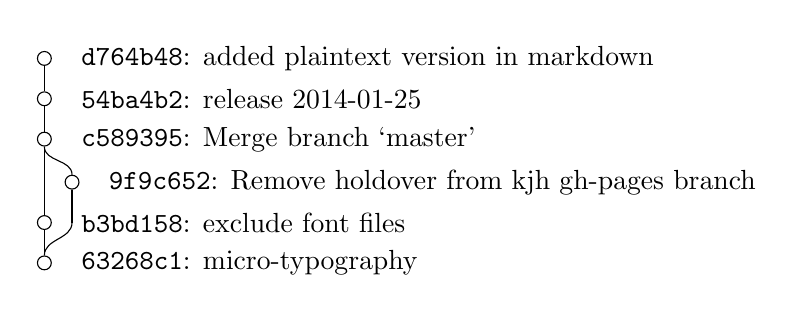
\begin{tikzpicture}
\tikzstyle{commit}=[draw,circle,fill=white,inner sep=0pt,minimum size=5pt]
\tikzstyle{clabel}=[right,outer sep=1em]
\tikzstyle{every path}=[draw]
\matrix [column sep={1em,between origins},row sep=\lineskip]
{
\commit{d764b48}{added plaintext version in markdown} & \\
\commit{54ba4b2}{release 2014-01-25} & \\
\commit{c589395}{Merge branch `master'} & \\
 & \commit{9f9c652}{Remove holdover from kjh gh-pages branch} \\
\commit{b3bd158}{exclude font files} & \ghost{branch1} \\
\commit{63268c1}{micro-typography} & \\
};
\connect{63268c1}{b3bd158};
\connect{63268c1}{branch1};
\connect{branch1}{9f9c652};
\connect{b3bd158}{c589395};
\connect{9f9c652}{c589395};
\connect{c589395}{54ba4b2};
\connect{54ba4b2}{d764b48};
\end{tikzpicture}


\begin{oceanbox}{3 way - merge と fast forward merge の使い分け}
With the 'enhanced' skin, it is quite easy to produce fancy looking effects.
\tcblower
Note that ...
\end{oceanbox}


\begin{oceanbox}{rebase と merge の使い分け}
With the 'enhanced' skin, it is quite easy to produce fancy looking effects.
\tcblower
Note that ...
\end{oceanbox}

% subsubsection merge (end)
\subsubsection{コミットメッセージの変更} % (fold)
\label{ssub:コミットメッセージの変更}

直前のcommit messageを変更するには以下を実行すれば良い。
\begin{commandshell}
git commit --amend
\end{commandshell}

2つ以上前のcommit messageを変更する場合には以下のようになる。

\begin{tcolorbox}[skin=enhanced,
left=3mm,right=3mm,top=1mm,bottom=1mm, boxrule=1.0mm, 
title=2つ以上前のcommit messageの変更, coltitle=black, fonttitle=\bfseries, 
colback=SpringGreen!5!white,colframe=SpringGreen!70]
n個前のcommit messageを変更したいとする。\\
\\
Step1. 変更対象のbranchにcheckoutし、以下を実行する
\begin{commandshell}
git rebase --interactive HEAD~n
\end{commandshell}

Step2. 変更したい対象のcommitのcommit idの隣の「pick」という文字を「edit」に書き換え
最初のeditの部分に戻っているので、以下を実行する
\begin{commandshell}
git commit --amend
\end{commandshell}

Step3. commit messageを変更後、以下を実行する
\begin{commandshell}
git rebase --continue
\end{commandshell}

Step4. 以降、editに書き換えた部分に対し、Step2, Step3を繰り返す\\
\\
Step5. git logを実行し、変更が反映されていることを確認する
\end{tcolorbox}


% subsubsection コミットメッセージの変更 (end)
\subsubsection{ブランチの削除} % (fold)
\label{ssub:ブランチの削除}

branchの削除の仕方については以下の2種類がある。\\
元になっているブランチよりも新しいcommitがある場合には、dオプションではerrorを返す。
\begin{commandshell}
git branch -d [target branch]
git branch -D [target branch]   # by force
\end{commandshell}

% subsubsection ブランチの削除 (end)


% subsection その他の使用頻度の高いコマンド (end)
%%%%%%%%%%%%%%%%%%%%%%%%%%%%%%%%%%%%%%%%%%%%%%%%%%%%


% section 基礎コマンド (end)
%%%%%%%%%%%%%%%%%%%%%%%%%%%%%%%%%%%%%%%%%%%%%section%%%%%%%%%%%%%%%%%%%%%%%%%%%%%%%%%%%%%%%%%%%%%%%%
\end{document}



% MIT License
% 
% sec4/section4.tex
% 
% Copyright (c) 2020 冬ノ夜空
% 

\documentclass[10pt,a4j,openany,dvipdfmx]{jsarticle}
\usepackage{docmute} %for "input" command

  % -- page layput
  \usepackage[top=3cm, bottom=3cm, left=3.5cm, right=2cm, includefoot]{geometry}

  % -- page configuration
  \renewcommand{\baselinestretch}{0.95} %行送りの倍率
  \renewcommand{\figurename}{Fig. }
  \renewcommand{\tablename}{Table. }

  % \renewcommand{\prepartname}{\Huge{Part\,}}
  % \renewcommand{\postpartname}{}
  % \renewcommand{\prechaptername}{Chapter\,}
  % \renewcommand{\postchaptername}{}

  %% \setlength{\hoffset}{4.6mm}
  %% \setlength{\marginparwidth}{0mm}

  % -- HyperLink
  \usepackage{url}
  \usepackage[dvipdfmx,bookmarks=true,bookmarksnumbered=true,colorlinks=true,linkcolor=MidnightBlue,urlcolor=MidnightBlue]{hyperref}
%  \usepackage[dvipdfmx,bookmarks=true,bookmarksnumbered=true,colorlinks=true,linkcolor=MidnightBlue,citecolor=MidnightBlue,urlcolor=MidnightBlue]{hyperref}

  % -- font
  \usepackage{bm}       %Italicな太字にする
  \usepackage{ulem}     % underlining for emphasis
  \usepackage{ascmac}   % "itembox" environment etc.

  \usepackage[T1]{fontenc}
  \usepackage{lmodern}   % Latin Modern フォントを使う
  \usepackage{courier}   % Courier typewriter フォント

  \usepackage{pxjahyper} %しおり・タイトル等の日本語の文字化け防止
  \usepackage{natbib}    %citeの強化版
  \bibliographystyle{ametsoc2014}

  % -- graphics / color
  \usepackage{graphicx}
  \usepackage{color}
  \usepackage{multicol}
  \usepackage[dvipdfmx,svgnames]{xcolor} %色の指定のためのパッケージ
  % \usepackage[dvipdfmx,dvipsnames]{xcolor} %色の指定のためのパッケージ

  % -- figure
  \usepackage{here}

  \usepackage{lscape}    % 図や表の回転
  \usepackage{pdflscape} % 自動的にLandscapeのページのみ回転してくれる

  \usepackage{enumitem}  % item環境のconfig.
    \setlist[description]{parsep=0mm,topsep=1mm,leftmargin=5mm}
    \setlist[itemize]{parsep=0mm,topsep=1mm,leftmargin=5mm}

  %background-image(all pages => \***; specific page => \This***)
  \usepackage{wallpaper}

  % -- symbol
  \usepackage{textcomp} % 様々なシンボル(特殊文字)を利用
                        % °は \degree、℃は \celsius を使う

  % 丸数字
  \newcommand{\maru}[1]{\lower0.5ex\hbox{{\Large \textcircled{\scriptsize{\raise0.5ex\hbox{\normalsize #1}}}}}}



%=========================================
% \usepackage{tocbibind}
% This option loads package tocbibind if not already done and so list of figures and list of tables are also added in the toc
% \usepackage{dotocloa} % Add algrism list into toc

\usepackage{tikz}
\usepackage{pxpgfmark}
  \usetikzlibrary{fit,calc}

  \usetikzlibrary{shadings} %for shading frame

%define a marking command
\newcommand*{\tikzmk}[1]{
\tikz[remember picture,overlay,] \node (#1) {};\ignorespaces
}

%define a boxing command, argument = colour of box
\newcommand{\boxit}[1]{
\tikz[remember picture,overlay]{\node[yshift=3pt,fill=#1,opacity=.25,fit={(A)( $(B)+(.95\linewidth,.8\baselineskip)$ )}] {};}\ignorespaces
}

%=========================================
% tcolorbox

\usepackage{tcolorbox}
  \tcbset{boxrule=0.3mm,left=1mm,right=1mm,top=1mm,bottom=1mm,boxsep=1.5mm}
  \newcommand{\defaultset}{\tcbset{colframe=Black!70!White,colback=White}}\defaultset

% newcommnd operation for tcolorbox
\newtcolorbox{forsomeone}[1]{fonttitle=\sffamily,title=#1}
\newtcbox{term}{colback=Red!10,left=1mm,right=1mm,top=1mm,bottom=1mm,before skip=2mm, after skip=2mm}\newcommand{\terminal}[1]{\texttt{\term{#1}}} %別行のターミナルコマンド
\newtcbox{inlineterm}{on line, colframe=Red!50!White, colback=Red!10,left=0.5mm,right=0.5mm,top=0.5mm,bottom=0.5mm,left skip=0.5zw, right skip=0.5zw,boxrule=0.2mm}\newcommand{\ilterm}[1]{\texttt{\inlineterm{#1}}} %行内のターミナルコマンド

\tcbuselibrary{listings}
% \newtcblisting{myverbatim}{listing only,colback=Black!5,before skip=2mm, after skip=2mm}
% \newtcblisting{multiterm}{listing only,colback=Red!10,before skip=2mm, after skip=2mm}

%\tcbuselibrary{skins}
\tcbuselibrary{many}

\newenvironment{blueitemize}{\begin{itemize}}{\end{itemize}}
\tcolorboxenvironment{blueitemize}{blanker,
left skip=10pt,left=10mm,
before skip=6pt,after skip=6pt,
borderline west={3mm}{0pt}{DeepSkyBlue}}


% \tcbset{skin=enhanced,fonttitle=\bfseries,
% frame style={upper left=Blue,upper right=Red,lower left=Yellow,lower right=Green},
% interior style={white,opacity=0.5},
% segmentation style={black,solid,opacity=0.2,line width=1pt}}

% \begin{tcolorbox}[title=Nice box in rainbow colors]
% With the 'enhanced' skin, it is quite easy to produce fancy looking effects.
% \tcblower
% Note that this is still a \texttt{tcolorbox}.
% \end{tcolorbox}

\makeatletter
  \newtcolorbox{picturebox}[2][]{%
  skin=enhanced, boxrule=1.0mm, fonttitle=\bfseries, 
  frame hidden, interior hidden, 
  overlay={\begin{tcbclipframe}\node at (frame)
  {\includegraphics[width=\tcb@width,height=\tcb@height]{#2}};\end{tcbclipframe}
  \begin{tcbclipinterior}\fill[white,opacity=0.75]
  (frame.south west) rectangle (frame.north east);\end{tcbclipinterior}},#1}
\makeatother


\newenvironment{oceanbox}[1]{\tcolorbox[savedelimiter=oceanbox,
skin=enhanced,boxrule=1.0mm,fonttitle=\bfseries,
frame style={upper left=Black,upper right=White,lower left=DeepSkyBlue,lower right=MidnightBlue},
interior style={white,opacity=0.5},
segmentation style={black,solid,opacity=0.2,line width=1pt},
title=#1]
} {\endtcolorbox}

\newenvironment{skybox}[1]{\tcolorbox[savedelimiter=skybox,
skin=enhanced,boxrule=1.0mm,fonttitle=\bfseries,
frame style={upper left=Black,upper right=White,lower left=Cyan,lower right=DodgerBlue},
interior style={white,opacity=0.5},
segmentation style={black,solid,opacity=0.2,line width=1pt},
title=#1]
} {\endtcolorbox}

\newenvironment{redbox}[1]{\tcolorbox[savedelimiter=redbox,
skin=enhanced,boxrule=1.0mm,fonttitle=\bfseries,
frame style={upper left=DarkRed,upper right=White,lower left=Black!50!DarkRed,lower right=Maroon},
interior style={white,opacity=0.5},
segmentation style={black,solid,opacity=0.2,line width=1pt},
title=#1]
} {\endtcolorbox}

\newtcolorbox{ColorReferenceBox}[1]{textmarker/.style={%
skin=enhancedmiddle jigsaw,breakable,parbox=false,
boxrule=0mm,leftrule=3mm,rightrule=3mm,boxsep=0mm,arc=0mm,outer arc=0mm,
left=3mm,right=3mm,top=1mm,bottom=1mm,toptitle=1mm,bottomtitle=1mm},
textmarker,colback=#1!5!white,colframe=#1}

% listing with line number
\newtcblisting{numList}[1]{
colback=red!5!white,colframe=red!25,
left=6mm, listing only,
listing options={style=tcblatex,language=#1,numbers=left,numberstyle=\tiny\color{red!75!black}}}

%=========================================
% commandshell, commandbox

  % color definition
  \definecolor{gentooblack}{HTML}{333333}
  
  % root user shell
  % *** Caution: 日本語を扱うのが苦手のよう!!!***
  \newtcblisting{rootshell}{boxrule=0.1mm,
  colback=gentooblack,colupper=white,colframe=DeepSkyBlue!95!white,
  listing only,listing options={style=tcblatex,language=sh},
  every listing line={\textcolor{red}{\small\ttfamily\bfseries [root]\# }}}
  
  % normal user shell
  % *** Caution: 日本語を扱うのが苦手のよう!!!***
  \newtcblisting{commandshell}{boxrule=0.1mm,
  colback=gentooblack,colupper=white,colframe=DeepSkyBlue!95!white,
  listing only,listing options={style=tcblatex,language=sh,columns=fullflexible,keywordstyle=\color{cyan}},
  every listing line={\textcolor{red}{\small\ttfamily\bfseries [user]\$ }}}

  \newtcblisting{onecommandshell}{boxrule=0.1mm,
  colback=gentooblack,colupper=white,colframe=DeepSkyBlue!95!white,
  listing only,listing options={style=tcblatex,columns=fullflexible}}

  % \usepackage{listings} or \tcbuselibrary{listings}
  \DeclareTotalTCBox{\commandbox}{ s v }
  {verbatim,colupper=white,colback=black!75!white,colframe=black}
  {\IfBooleanTF{#1}{\textcolor{red}{\ttfamily\bfseries > }}{}%
  \lstinline[language=command.com,keywordstyle=\color{cyan!35!white}\bfseries]^#2^}

%=========================================

% for drawing the git flow diagram
\usepackage{filecontents} 
\newcommand\commit[2]{\node[commit] (#1) {}; \node[clabel] at (#1) {\texttt{#1}: #2};}
\newcommand\ghost[1]{\coordinate (#1);}
\newcommand\connect[2]{\path (#1) to[out=90,in=-90] (#2);}

%=========================================

\usepackage{listings}
\lstset{
  language = , %プログラム言語(複数の言語に対応,C,C++も可)(plain textの場合は言語設定を空にする!!!)
  %backgroundcolor={\color{White}},                   %背景色と透過度
  breaklines = true,                                 %枠外に行った時の自動改行
  breakindent = 10pt,                                %自動改行後のインデント量(デフォルトでは20[pt])
  basicstyle = \ttfamily\scriptsize,                 %標準の書体
  commentstyle = {\itshape \color[cmyk]{1,0.4,1,0}}, %コメントの書体
  classoffset = 0,                                   %関数名等の色の設定
  keywordstyle = {\bfseries \color[cmyk]{0,1,0,0}},  %キーワード(int, ifなど)の書体
  stringstyle = {\ttfamily \color[rgb]{0,0,1}},      %表示する文字の書体
  %frame = TBrl,       %枠 "t"は上に線を記載, "T"は上に二重線を記載 
                       %他オプション:leftline,topline,bottomline,lines,single,shadowbox
  framesep = 5pt,      %frameまでの間隔(行番号とプログラムの間)
  numbers = none,      %行番号の位置 (行番号無し:none; 左:left; 右:right)
  stepnumber = 1,      %行番号の間隔
  numberstyle = \tiny, %行番号の書体
  tabsize = 4,         %タブの大きさ
  captionpos = t       %キャプションの場所("tb"ならば上下両方に記載)
}
%% Color Numbers
%\lstset
%{
%    literate=%
%    {0}{{{\color{Orange}0}}}1
%    {1}{{{\color{Orange}1}}}1
%    {2}{{{\color{Orange}2}}}1
%    {3}{{{\color{Orange}3}}}1
%    {4}{{{\color{Orange}4}}}1
%    {5}{{{\color{Orange}5}}}1
%    {6}{{{\color{Orange}6}}}1
%    {7}{{{\color{Orange}7}}}1
%    {8}{{{\color{Orange}8}}}1
%    {9}{{{\color{Orange}9}}}1
%}

  %\usepackage{layout} % layout図を表示するためのパッケージ
  %  \setlength{\voffset}{-0.5in} % headerの高さ
  %  \setlength{\headheight}{1zw} % headerの高さ
  %  \setlength{\textheight}{42\baselineskip} % textboxの高さ.
  %  \setlength{\textwidth}{\fullwidth} % textboxの幅.
  %  \setlength{\evensidemargin}{\oddsidemargin} % 左右の欄外枠の幅をwordっぽくする
  %  \setlength{\footskip}{4zw}
  %  \setlength{\parindent}{0pt} %global に\noindent
  %  \setlength{\parskip}{0.5\baselineskip}
  %  \setlist[itemize]{leftmargin=12pt}

%=========================================

  %DRAFTという斜め文字を入れていた原因
  %\usepackage{draftwatermark}

  \usepackage{mathcomp}
  \usepackage{amsmath,amssymb}
% \usepackage{mathptmx} %A,Bのmathcal の別のfontを使う

  \usepackage[ruled]{algorithm2e} % http://www.ctan.org/pkg/algorithm2e
    \LinesNumbered % Add Line Numbers

  %define some colors according to algorithm parts (or any other method you like)
  \colorlet{pink}{red!40}
  \colorlet{blue}{cyan!60}
  \colorlet{mint}{green!40}


  \newtheorem{thm}{定理}[section]%paper_3のために書いている(paper_3を消すときに消せばいい)
  \newtheorem{lem}[thm]{補題}
  \newtheorem{axm}[thm]{公理}
  

  \newcommand{\todaye}{\the\year{\text 年}\the\month{\text 月}}
  % \newcommand{\terminal}[1]{%
  % \\\hspace{3zw}\colorbox{Red!20}{\texttt{#1}}\\%
  % }
  \newcommand{\whiteterminal}[1]{%
  \\\hspace{3zw}\texttt{#1}\\%
  }
  \newcommand{\textbtt}[1]{\textbf{\texttt{#1}}} %太字のコマンド表示、ここではディレクトリ名に用いる
  \newcommand{\blueunder}[1]{\textcolor[rgb]{0,0,1}{\underline{#1}}}%下線と青字を施す

%=========================================

\usepackage{varwidth}
\newtcolorbox{myfilebox}[2][]{enhanced,
before skip=2mm,after skip=2mm,
colback=black!5,colframe=black!50,boxrule=0.2mm,
attach boxed title to top left={xshift=1cm,yshift*=1mm-\tcboxedtitleheight},
varwidth boxed title*=-3cm,
boxed title style={frame code={
\path[fill=tcbcolback!30!black]
([yshift=-1mm,xshift=-1mm]frame.north west)
arc[start angle=0,end angle=180,radius=1mm]
([yshift=-1mm,xshift=1mm]frame.north east)
arc[start angle=180,end angle=0,radius=1mm];
\path[left color=tcbcolback!60!black,right color=tcbcolback!60!black,
middle color=tcbcolback!80!black]
([xshift=-2mm]frame.north west) -- ([xshift=2mm]frame.north east)
[rounded corners=1mm]-- ([xshift=1mm,yshift=-1mm]frame.north east)
-- (frame.south east) -- (frame.south west)
-- ([xshift=-1mm,yshift=-1mm]frame.north west)
[sharp corners]-- cycle;
},interior engine=empty,
},
fonttitle=\bfseries,
title={#2},#1}

%=========================================




\begin{document}

%%%%%%%%%%%%%%%%%%%%%%%%%%%%%%%%%%%%%%%%%%%%%section%%%%%%%%%%%%%%%%%%%%%%%%%%%%%%%%%%%%%%%%%%%%%%%%
\section{Deep Dive} % (fold)
\label{sec:Deep Dive}


%%%%%%%%%%%%%%%%%%%%%%%%%%%%%%%%%%%%%%%%%%%%%%%%%%%%
\subsection{役に立つコマンド} % (fold)
\label{sub:役に立つコマンド}


\subsubsection{cherry-pick} % (fold)
\label{ssub:cherry_pick}

他のブランチなどにあるcommitも取り込むことができる。\\
取り込みたいbranchにcheckoutし、その後、取り込みたいcommit idを羅列するだけで良い。
\begin{commandshell}
git checkout [target branch]
git cherry-pick [target commit 1] [target commit 2] ...
\end{commandshell}

詳細は以下を参照。
cherry-pick: \url{https://git-scm.com/docs/git-cherry-pick}

% subsubsection cherry_pick (end)
\subsubsection{tag} % (fold)
\label{ssub:tag}

特定のcommitに対してv1.0というタグをつけたい場合は以下のように実行する。
\begin{commandshell}
git tag v1.0 [target commit id]
git tag -m "version 1.0" v1.0 [target commit id]   # with a comment
\end{commandshell}

現在のタグを確認する場合は、以下を実行すれば良い。
\begin{commandshell}
git tag
\end{commandshell}

詳細は、以下を参照。
tag: \url{https://git-scm.com/book/en/v2/Git-Basics-Tagging}

% subsubsection tag (end)
\subsubsection{show} % (fold)
\label{ssub:show}

特定のcommitの変更内容を表示できる。最新のcommitの変更内容を表示するには以下を実行する。
\begin{commandshell}
git show HEAD
\end{commandshell}

% subsubsection show (end)
\subsubsection{clean} % (fold)
\label{ssub:clean}

\begin{commandshell}
git clean -n
git clean -f 
\end{commandshell}

% subsubsection clean (end)
\subsubsection{archive} % (fold)
\label{ssub:archive}

\$ git archive --format=tar --prefix=[directory name] HEAD | \
gzip > [directory path]/[file name].tar.gz

prefixオプションで、展開後のディレクトリを指定できる。

% subsubsection archive (end)
\subsection{hunk単位でのオペレーション} % (fold)
\label{sub:hunk単位でのオペレーション}

\begin{tcolorbox}[title=hunkとは, fonttitle=\bfseries]
管理対象のファイルに対し、Gitはブロック単位でコードを認識している。
hunkとは、コード内におけるGitが認識するブロックのことである。
\end{tcolorbox}

以下ではhunk単位での扱いについて記載する。

hunk単位でのindexへの登録
\begin{commandshell}
git add -p
\end{commandshell}

hunk単位でのcommit
\begin{commandshell}
git commit --interactive
\end{commandshell}

% subsection hunk単位でのオペレーション (end)

% subsection 役に立つコマンド (end)
%%%%%%%%%%%%%%%%%%%%%%%%%%%%%%%%%%%%%%%%%%%%%%%%%%%%
\subsection{もっと学びたい方へ} % (fold)
\label{sub:もっと学びたい方へ}


\begin{skybox}{Git Branch Model}
Git Branch Modelというものを学習すると良いだろう。
Git-Flow, GitHub-Flowなどが存在する。
\tcblower
\url{https://nvie.com/posts/a-successful-git-branching-model/}
\end{skybox}

\begin{redbox}{ProGit}
ProGitという本がGit本家から出ているので、より詳しく学びたい場合は一読すると良いだろう。
\tcblower
Git HP: \url{https://git-scm.com/book/en/v2}
GitHub: \url{https://github.com/progit/}
\end{redbox}


% subsection もっと学びたい方へ (end)
%%%%%%%%%%%%%%%%%%%%%%%%%%%%%%%%%%%%%%%%%%%%%%%%%%%%


% section Deep Dive (end)
%%%%%%%%%%%%%%%%%%%%%%%%%%%%%%%%%%%%%%%%%%%%%section%%%%%%%%%%%%%%%%%%%%%%%%%%%%%%%%%%%%%%%%%%%%%%%%
\end{document}




% Reference
\bibliography{./ref/reference}

\end{document}


